%=== How to use:
%   \confvertrue, \plainverfalse = 2 column IEEE version
%   \confverfalse, \plainverfalse = 1 column IEEE draft version
%   \plainvertrue = our plain version

\newif\ifconfver
%\confverfalse      %declaring conference version false
\confvertrue        %declaring conference version true

\newif\ifonecoltab
\onecoltabtrue        % declaring one column version table size true
%\onecoltabfalse

\newif\ifplainver  %declare a plain version
%\plainvertrue
%\plainverfalse

\ifplainver
    \confverfalse                         %automatically disable conf. version argument if it's plain
\fi

\ifconfver
     \documentclass[10pt,journal]{IEEEtran}
\else
    \ifplainver
        \documentclass[11pt]{article}
        \usepackage{fullpage}
    \else
        \documentclass[12pt,draftcls,onecolumn]{IEEEtran}
    \fi
\fi




\usepackage{calc,amsfonts,amssymb,amsmath,bm,url,color,theorem,graphicx,cite,epstopdf,nicefrac}
\usepackage{psfrag,subfigure,float}
\usepackage[algoruled,linesnumbered]{algorithm2e}
\usepackage{multirow}
%\usepackage{algorithm}
%\usepackage{algorithmic}
\usepackage[normalem]{ulem}

%--- define color
\definecolor{orange}{RGB}{255,107,0}
\def\blue{\color{blue}}
\def\red{\color{red}}
\def\orange{\color{orange}}
\def\green{\color{green}}

%--- defining the theorem and stuff

\newtheorem{Fact}{Fact}
\newtheorem{Lemma}{Lemma}
\newtheorem{Prop}{Proposition}
\newtheorem{Theorem}{Theorem}
\newtheorem{Def}{Definition}
\newtheorem{Corollary}{Corollary}
\newtheorem{Property}{Property}
\newtheorem{Observation}{Observation}
\theorembodyfont{\rmfamily}
\newtheorem{Exa}{Example}
\newtheorem{Assumption}{Assumption}
\newtheorem{Remark}{Remark}


%make sure to keep this for convenience later
\newcommand\bd{\ensuremath{{\rm bd}}}
\newcommand\inte{\ensuremath{{\rm int}}}
%---- vectors -----------------
\newcommand{\vct}{\bm{t}}
\newcommand{\vcx}{\bm{x}}
%---- sets --------------------
\newcommand{\setB}{\mathcal{B}}
\newcommand{\setR}{\mathcal{R}}
\newcommand{\setW}{\mathcal{W}}
\newcommand{\Rbb}{\mathbb{R}}
\newcommand{\MVES}{\mathsf{MVES}}





\newcommand{\W}{\boldsymbol{W}}
\newcommand{\G}{\boldsymbol{G}}
\newcommand{\Q}{\boldsymbol{Q}}
\newcommand{\X}{\boldsymbol{X}}
\newcommand{\C}{\boldsymbol{C}}
\newcommand{\E}{\boldsymbol{E}}
\newcommand{\U}{\boldsymbol{U}}
\newcommand{\K}{\mathcal{K}}
\newcommand{\one}{\boldsymbol{1}}
\newcommand{\M}{\boldsymbol{M}}
\newcommand{\A}{\boldsymbol{A}}
\newcommand{\B}{\boldsymbol{B}}
\newcommand{\x}{\boldsymbol{x}}
\newcommand{\m}{\boldsymbol{m}}
\renewcommand{\a}{\boldsymbol{a}}
\renewcommand{\th}{\boldsymbol{\theta}}

%%%%%%%%%%%%%%%%%%%%%%%%%%%%%%%%%%%%%%%%%%%%%%%%%%%%%%%%%%%%%%%%%%%%%%%%%%%%%%%
% From Nikos: reminder command:
\newcommand{\reminder}[1]{ \color{blue} [[[ \marginpar{\mbox{\color{blue} ${\bf <==}$ \color{black}}} #1 ]]] \color{black}}
%\newcommand{\reminder}[1]{} % do not show reminders
%%%%%%%%%%%%%%%%%%%%%%%%%%%%%%%%%%%%%%%%%%%%%%%%%%%%%%%%%%%%%%%%%%%%%%%%%%%%%%%

% correct bad hyphenation here
\hyphenation{op-tical net-works semi-conduc-tor}


\begin{document}

\bibliographystyle{IEEEtran}

%--- I do things quite strangely here to accommodate three style modes.
%--- input title and abstract here; it applies to all modes
%--- it's too complex to do authors or they are input for each mode
\newcommand{\papertitle}{
%Robust Volume Minimization-Based Matrix Factorization for Remote Sensing and Document Clustering
Scalable and Flexible Multiview Canonical Correlation Analysis
}

\newcommand{\paperabstract}{
This paper considers generalized (multiview) canonical correlation analysis (GCCA) for large-scale datasets.
A memory-efficient and computationally lightweight algorithmic framework is proposed for the classic MAX-VAR GCCA formulation as well as its variants.
GCCA is gaining renewed interest in various applications such as speech processing and natural language processing. The classic MAX-VAR GCCA problem can be solved optimally via eigen-decomposition of a matrix that compounds the (whitened) correlation matrices of the views. 
However, this route can easily lead to memory explosion and a heavy computational burden when the size of the views becomes large. 
In addition, it was unclear how to compute structured canonical components under the MAX-VAR formulation, which are often desired in data analytics -- e.g., sparse canonical components are
favorable in many applications since they have the effect of avoiding outlying data.
To address the above issues,
we propose an alternating optimization (AO)-based algorithm, which avoids instantiating the correlation matrices of the views and thus can achieve substantial saving in memory. The algorithm also maintains data sparsity, which can be exploited to alleviate the computational burden. Consequently, the proposed algorithm is highly scalable. 
Regularization such as sparsity promoting functions can be easily incorporated in the proposed computational framework. 
Convergence properties of the proposed algorithm are carefully studied.
Simulations and large-scale word embedding tasks are employed to showcase the effectiveness of the proposed algorithm.
}

%--------

\ifplainver

    \date{\today}

    \title{\papertitle}

    \author{
    Xiao Fu$^\ast$, Kejun Huang$^\ast$, Mingyi Hong	$^\ddag$, Nicholas D. Sidiropoulos$^\ast$, and Anthony Man-Cho So$^\dag$
    \\ ~ \\
		$^\ast$Department of Electrical and Computer Engineering, University of Minnesota,\\
		Minneapolis, 55455, MN, United States\\
		Email: (xfu,huang663,nikos)@umn.edu
	  \\~\\
	$^\ddag$Department of Industrial and Manufacturing Systems Engineering, Iowa State University\\
	Ames, Iowa 50011, (515) 294-4111,\\
	Email: mingyi@iastate.edu
	 \\ ~ \\
    $^\dag$Department of Systems Engineering and Engineering Management\\ The Chinese University of Hong Kong, \\
	Shatin, N.T., Hong Kong \\
	Email: manchoso@se.cuhk.edu.hk 
	\\
    }

    \maketitle
	

    \begin{abstract}
    \paperabstract
    \end{abstract}

\else
    \title{\papertitle}

    \ifconfver \else {\linespread{1.1} \rm \fi

   \author{Xiao Fu, Kejun Huang, Mingyi Hong,  Nicholas D. Sidiropoulos, and Anthony M.-C. So
\thanks{X. Fu, K. Huang and N.D. Sidiropoulos are with the Department of Electrical and Computer Engineering, University of Minnesota, Minneapolis, MN55455, e-mail (xfu,huang663,nikos)@umn.edu.
M. Hong is with Department of Industrial and Manufacturing Systems Engineering, Iowa State University,	Ames, Iowa 50011, (515) 294-4111, Email: mingyi@iastate.edu.
Anthony M.-C. So is with the Department of Systems Engineering and Engineering Management, The Chinese University of Hong Kong, Shatin, N.T., Hong Kong, Email: manchoso@se.cuhk.edu.hk 
}
}

    \maketitle

    \ifconfver \else
        \begin{center} \vspace*{-2\baselineskip}
        %11th Revision, \today \\[2\baselineskip]
        \end{center}
    \fi

    \begin{abstract}
    \paperabstract
    \end{abstract}

%    \begin{keywords}\vspace{-0.0cm}
%        Simplex-volume minimization, identifiability, matrix factorization, robustness against outliers, hyperspectral unmixing, document clustering
%    \end{keywords}

    \ifconfver \else \IEEEpeerreviewmaketitle} \fi

 \fi

\ifconfver \else
    \ifplainver \else
        \newpage
\fi \fi
%---------------------------------------------------------------------------


  
	

%---------------------------------------------------------------------------
\section{Introduction}
Canonical Correlation Analysis (CCA) \cite{hardoon2004canonical} produces low dimensional representations by finding common structure of two or more views corresponding to the same entities.
A view contains high-dimensional representations of the entities in some domain -- e.g., the text and audio representations corresponding to a given word can be considered as different views of this word.
CCA is able to deal with views that have different dimensions, and this flexibility is very useful in data fusion, where one is interested in integrating information gathered from different domains.
Multiview analysis finds numerous applications in machine learning, such as regression \cite{kakade2007multi}, clustering \cite{chaudhuri2009multi}, speech modeling and recognition \cite{arora2014multi,wang2015acoustic}, and word embedding \cite{rastogimultiview}, to name a few.
Classical CCA was derived for the two-view case, but Generalized Canonical Correlation Analysis (GCCA) that aims at handling more than two views has a long history as well \cite{carroll1968generalization}.
A typical application of GCCA is word embedding in natural language processing, where the vocabularies from different languages can be considered as multiple views of the same terms.
Word embedding seeks low-dimensional representations of the terms that are well-aligned with human judgment, and applying GCCA to integrate multiple languages was shown to yield better embedding results relative to single-view analyses such as principle component analysis (PCA) \cite{rastogimultiview}.

Computationally, GCCA poses interesting and challenging optimization problems.
Unlike the two-view case that admits an algebraically simple solution (via eigen-decomposition),
GCCA is in general not easily solvable.
Many prior works considered the GCCA problem with different cost functions \cite{carroll1968generalization,kettenring1971canonical}, while the proposed algorithms often can only extract a single canonical component and then find others through a deflation process, which is known to suffer from error propagation.
Convergence properties of the GCCA algorithms are also largely under-investigated, since
the GCCA formulations often involve non-convex constraints (e.g., manifold constraints) that complicate analysis.
CCA and GCCA can also pose serious scalability challenges,
since they involve auto- and cross-correlations of different views and a whitening stage \cite{ma2015finding}.
These procedures can easily lead to memory explosion and require a large number of flops for computation.
They also destroy the sparsity of the data, which is usually what one relies upon to deal with large-scale problems.
In recent years, effort has been spent on solving these scalability issues, but the focus is mostly on the two-view case \cite{ma2015finding,sun2011canonical,lu2014large}.

Besides the basic (G)CCA formulations, \emph{structured} CCA \cite{hardoon2011sparse} is often considered in applications.
For example, sparse CCA is often considered in data analytics, for the purpose of discarding irrelevant features when performing CCA \cite{witten2009penalized,chen2012structured,witten2009extensions}.
%In multi-lingual word embedding \cite{faruqui2014improving,sun2011canonical,rastogimultiview}, for example, it is known that there are many irrelevant features, such as stop words. In brain activation analysis, it is also believed that many voxels are irrelevant and should be somehow discarded \cite{rustandi2009integrating,mitchell2008predicting}. Gene analysis is another example \cite{witten2009penalized,chen2012structured,witten2009extensions}.
Ideally, CCA seeks a few highly correlated latent components, and so it should naturally be able to identify and down-weight irrelevant features automatically. In practice, however, this ability is often impaired when correlations cannot be reliably estimated, when one only has access to relatively few and/or very noisy samples, or when there is model mismatch due to bad preprocessing (e.g., registration). In those cases, performing feature selection jointly with (G)CCA is well-motivated. However, introducing structure regularizations on the sought canonical components makes the optimization problem even harder -- since many regularization terms like the sparsity-promoting regularizers are non-differentiable.

Among all different formulations of GCCA, there is a particular one that admits a conceptually simple solution, the so-called MAX-VAR GCCA \cite{carroll1968generalization,van2006generalized,kettenring1971canonical}.
MAX-VAR GCCA was first proposed in \cite{carroll1968generalization}, and its solution amounts to finding the `directions' aligned to those exhibiting maximum variance for a matrix aggregated from the (whitened) auto-correlations of the views.
It can also be viewed as a problem of enforcing {\em identical} latent representations of different views as opposed to highly correlated ones, which is the more general goal of (G)CCA.
The merit of MAX-VAR GCCA is that it can be solved via eigen-decomposition
and finds all the canonical components simultaneously (i.e., no deflation is involved).
In practice, MAX-VAR GCCA also demonstrates promising performance in various applications such as word embedding \cite{rastogimultiview} and speech recognition \cite{arora2014multi}.
On the other hand, MAX-VAR GCCA has the same scalability problem as the other GCCA formulations:
It involves correlation matrices of different views and their inverses, which is prohibitive to even instantiate when the data dimension is large.
The work in \cite{rastogimultiview} provided a pragmatic way to circumvent this difficulty: PCA was first applied to each view to reduce the rank of the views,
and then MAX-VAR GCCA was applied to the rank-truncated views. Such a procedure significantly reduces
the number of parameters for characterizing the views and is feasible in terms of memory. However, truncating the rank of the views is prone to information loss, and thus leads to performance degradation.
Another shortcoming of the algorithm in \cite{rastogimultiview} is that it cannot handle regularizations for structure promoting.

\bigskip

\noindent
{\bf Contributions}
In this work, our interest lies in solving the MAX-VAR GCCA problem and its variants when the dimensions of the views are large.
Instead of truncating the rank of the views as in \cite{rastogimultiview}, we keep the data \emph{intact} and devise a scalable algorithmic framework to handle the original MAX-VAR problem
and variants with structure-promoting regularizers.
Specifically, our idea is based on a two-block alternating optimization (AO) algorithm tailored for the considered problems.
Under the AO framework, the proposed algorithm alternates between a (regularized) least squares subproblem and an orthogonality-constrained subproblem.
The merit of this framework is that correlation matrices of the views never need to be explicitly instantiated, and the inversion procedure is avoided. 
Consequently, the algorithm consumes significantly less memory compared to that required by the original solution using eigen-decomposition.
The proposed algorithm is also very flexible in incorporating different structure-promoting regularizers.

On the theory side, convergence properties of the algorithm are also carefully studied:
We first show that the proposed algorithm \emph{globally} converges to a Karush-Kuhn-Tucker (KKT) point of the formulated problem under a variety of regularizers, even when the subproblems are solved in a grossly inexact manner.
We also show that the optimality gap shrinks to at most ${\cal O}(1/r)$ after $r$ iterations -- i.e.,
at least a sublinear convergence rate can be guaranteed.
In addition, we show that when there is no regularization, the proposed algorithm solves the MAX-VAR problem to \textit{global optimality} with a \textit{linear} convergence rate.
When the subproblems are not exactly solved, such a rate still holds with some loss in accuracy.
The proposed algorithm is applied to synthetic data and a real large-scale word embedding problem, and promising results are observed.

\bigskip

\noindent
{\bf Notation} We use $\X$ and ${\bm x}$ to denote a matrix and a vector, respectively.
$\X(m,:)$ and $\X(:,n)$ denote the $m$th row and the $n$th column of $\X$, respectively;
in particular, $\X(:,\ell_1:\ell_2)$ denotes a submatrix of $\X$ consisting of the $\ell_1$-$\ell_2$th columns of $\X$ (\texttt{MATLAB} notation).
$\|\X\|_F$ and $\|\X\|_p$ for $p\geq 1$ denote the Frobenius norm and the matrix-induced $p$-norm, respectively. $\|\X\|_{p,1} = \sum_{i=1}^m \|\X(i,:)\|_p$ for $p\geq 1$ denotes the $\ell_p\ell_1$-mixed norm of $\X\in\mathbb{R}^{m\times n}$.
The superscripts ``$T$'', ``$\dag$'', and ``${-1}$'' denote the matrix operators of transpose, pseudo-inverse and inverse, respectively. 

\section{Background}

The classic two-view CCA can be expressed as the following optimization problem \cite{hardoon2004canonical}:
\begin{equation}\label{eq:CCA}
\begin{aligned}
    \min_{{\bm Q}_1,{\bm Q}_2} &~\left\|{\bm X}_1{\bm Q}_1-{\bm X}_2{\bm Q}_2\right\|_F^2\\        
                                  {\rm s.t.} &~{\bm Q}_i^T\left({\bm X}_i^T{\bm X}_i\right){\bm Q}_i={\bm I},\quad i=1,2,
\end{aligned}
\end{equation}
where ${\bm X}_i\in\mathbb{R}^{L\times M_i}$, with its $\ell$th row ${\bm X}_i(\ell,:)$ containing the $i$th view of the $\ell$th data point, the columns of ${\bm Q}_i\in\mathbb{R}^{M_i\times K}$ correspond to the $K$ canonical components of view ${\bm X}_i$, and $(\nicefrac{1}{L}){\bm X}_i^T{\bm X}_i$ serves as an estimate of the correlation of each view.
%${\bm Q}_1$ and ${\bm Q}_2$ can be considered as two linear operators which 
%reduce the dimensionality of ${\bm X}_1$ and ${\bm X}_2$, respectively,
%so that the reduced-dimension views, i.e., ${\bm X}_i{\bm Q}_i$ for $i=1,2,$, are highly correlated
%-- since essentially we are maximizing the trace of the estimated cross-correlations between the views, i.e., ${\rm Tr}((\nicefrac{1}{L}){\bm Q}_2^T{\bm X}_2^T{\bm X}_1{\bm Q}_1$).
Note that we are essentially maximizing the trace of the estimated cross-correlations between the views, i.e., ${\rm Tr}( \bm{Q}_2^T\bm{X}_2^T\bm{X}_1\bm{Q}_1)$.  Thus, $\bm{Q}_1$ and $\bm{Q}_2$ can be considered as two linear operators that reduce the dimensionality of $\bm{X}_1$ and $\bm{X}_2$, respectively, so that the reduced-dimension views, i.e., $\bm{X}_i\bm{Q}_i$ for $i=1,2$, are highly correlated.
The constraints serve the purpose of normalization.
Problem~\eqref{eq:CCA} can be solved exactly via an (generalized) eigen-decomposition, but this simple solution only applies to the two-view case. To analyze the case with more than two views, the so-called generalized CCA (GCCA) is often adopted \cite{carroll1968generalization}. 
Different cost functions of GCCA were proposed \cite{kettenring1971canonical,tenenhaus2011regularized,carroll1968generalization,tenenhaus2014variable}, and arguably the most natural extension of CCA is the following \cite{hardoon2004canonical}:
\begin{equation}\label{eq:GCCA}
\begin{aligned}
\min_{\{{\bm Q}_i\}_{i=1}^I} &~\sum_{i=1}^{I-1}\sum_{j=i+1}^I\left\|{\bm X}_i{\bm Q}_i-{\bm X}_j{\bm Q}_j\right\|_F^2\\        
{\rm s.t.} &~{\bm Q}_i^T\left({\bm X}_i^T{\bm X}_i\right){\bm Q}_i={\bm I},~i=1,\ldots, I,
\end{aligned}
\end{equation}
where $I$ is the number of views.
Unfortunately, Problem~\eqref{eq:GCCA} does not admit an analytic solution.
Another formulation of GCCA is more tractable: Instead of forcing pairwise similarity of the reduced-dimension views,
one can seek a common latent representation of different views, i.e., \cite{carroll1968generalization,rastogimultiview,arora2014multi,van2006generalized,kettenring1971canonical}
\begin{equation}\label{eq:CGCCA}
\begin{aligned}
\min_{\{{\bm Q}_i\}_{i=1}^I,{\bm G}^T{\bm G}={\bm I}} &~\sum_{i=1}^{I}(\nicefrac{1}{2})\left\|{\bm X}_i{\bm Q}_i-{\bm G}\right\|_F^2,
\end{aligned}
\end{equation}
where ${\bm G}\in\mathbb{R}^{L\times K}$ is the common latent representation of the different views.
Conceptually, Problems~\eqref{eq:CGCCA} and \eqref{eq:GCCA} share the same goal, i.e., find highly correlated reduced-dimension views. On the other hand, the solutions may be different since the ${\bm X}_i {\bm Q}_i$'s yielded by Problem~\eqref{eq:CGCCA} are not forced to be exactly orthogonal, but only approximately so.
%enforces perfect correlation between the latent representations of the views \reminder{It tries to, but it may not be able to enforce perfect correlation ... Perhaps a clearer difference is that the ${\bf X}_i {\bf Q}_i$'s in Problem~\eqref{eq:CGCCA} are not forced to be exactly orthogonal, only approximately so.}.
The upshot of Problem~\eqref{eq:CGCCA} is that it admits a {\em conceptually} simple algebraic solution, which, as we will show, has the potential to be scaled up to deal with very large problems. %\reminder{Check edits I made in the previous sentence.} 
In this work, we will focus on Problem~\eqref{eq:CGCCA}.

Problem \eqref{eq:CGCCA} is referred to as the MAX-VAR formulation of GCCA since the optimal solution amounts to taking principal eigenvectors of a matrix aggregated from the correlation matrices of the views.
To explain, let us first assume that ${\bm X}_i$ has full column rank
and marginalize ${\bm Q}_i$ by letting
${\bm Q}_i=(\sqrt{L}){\bm X}_i^\dag{\bm G}$, where ${\bm X}_i^\dag=({\bm X}_i^T{\bm X}_i)^{-1}{\bm X}_i^T$. By substituting it back to \eqref{eq:CGCCA}, we see that an optimal solution ${\bm G}_{\rm opt}$ can be obtained via solving the following:
\begin{equation}
\begin{aligned}
{\bm G}_{\rm opt}=&\arg\min_{{\bm G}^T{\bm G}={\bm I}}~\sum_{i=1}^I\left\| {\bm G} - {\bm X}_i{\bm X}_i^\dag{\bm G} \right\|_F^2\\
& = \arg\max_{{\bm G}^T{\bm G} = {\bm I}} ~ {\rm Tr}\left({\bm G}^T\left(\sum_{i=1}^I {\bm X}_i{\bm X}_i^\dag\right){\bm G}\right). \label{eq:new_obj}
\end{aligned}
\end{equation}
Let ${\bm M} = \sum_{i=1}^I {\bm X}_i{\bm X}_i^\dag$.
Then, an optimal solution is ${\bm G}_{\rm opt}={\bm U}_M(:,1:K)$, 
%where ${\bm U}_M{\bm \Sigma}_M{\bm V}^T_M = {\rm svd}({\bm M})$ -- i.e., taking 
the first $K$ principal eigenvectors of ${\bm M}$ \cite{GHGolub1996}.

Although Problem~\eqref{eq:CGCCA} admits a seemingly easy solution, implementing it for large-scale data is prohibitive. 
The first difficulty lies in memory: As mentioned, instantiating ${\bm M} = \sum_{i=1}^I{\bm X}_i({\bm X}_i^T{\bm X}_i)^{-1}{\bm X}_i^T$ is not doable when $L$ and $M_i$'s are large. The matrix ${\bm M}$ is an $L\times L$ matrix. In applications like word embedding, $L$ and $M_i$ are the vocabulary size of a language and the number of features defining the terms, respectively, which can both easily exceed $100,000$. This means that the memory for simply instantiating ${\bm M}$ or $({\bm X}_i^T{\bm X}_i)^{-1}$ can reach 75GB.	
In addition, even if the views ${\bm X}_i$ are sparse, computing $({\bm X}_i^T{\bm X}_i)^{-1}$ will create large dense matrices and make it difficult to exploit sparsity in the subsequent processing.
To circumvent these difficulties, Rastogi \emph{et al.} \cite{rastogimultiview} proposed to first apply the singular value decomposition (SVD) to the views, i.e., ${\rm svd}({\bm X}_i)={\bm U}_i{\bm \Sigma}_i{\bm V}_i^T$, and then let 
	\[\hat{\bm X}_i = {\bm U}_i(:,1:P){\bm \Sigma}_i(1:P,1:P)({\bm V}_i(:,1:P))^T \approx {\bm X}_i,\]
where $P$ is much smaller than $M_i$ and $L$.
This procedure enables one to represent the views with significantly fewer parameters, i.e., $(L+M_i+1)P$ compared to $LM_i$,
and allows the original eigen-decomposition based solution to MAX-VAR GCCA to be applied; see more details in \cite{rastogimultiview}.	The drawback, however, is also evident: The procedure essentially truncates the rank of the views significantly (since in practice the views almost always have full column-rank, i.e., ${\rm rank}({\bm X}_i)=M_i$), and rank-truncation may lose a lot of information. Therefore, it is much more appealing to deal with the original views directly. 
Another shortcoming of the above approach is that it is not flexible in incorporating regularizations on $\Q_i$, while structured $\Q_i$ are often desired in different applications \cite{witten2009penalized,chen2012structured,witten2009extensions}.

In this work, we provide an algorithmic framework that deals with the MAX-VAR GCCA problem and its variants with constraints on $\Q_i$.
We aim at offering
simple solutions that are memory-efficient, admit light per-iteration complexity, and feature good convergence properties under certain mild conditions.
%Our algorithm allows one to exploit sparsity of large-scale data and is flexible in incorporating regularization.


\section{Proposed Algorithm}
In this work, we consider a scalable and flexible algorithmic framework for handling MAX-VAR GCCA and some variants. Specifically, we consider the following formulation
\begin{equation}\label{eq:CGCCA_reg}
\begin{aligned}
\min_{\{{\bm Q}_i\}_{i=1}^I,\G} &~\sum_{i=1}^{I}(\nicefrac{1}{2})\left\|{\bm X}_i{\bm Q}_i-{\bm G}\right\|_F^2+\sum_{i=1}^I  g_i(\Q_i),\\
{\rm s.t.}&~{\bm G}^T{\bm G}={\bm I},
\end{aligned}
\end{equation}
where $g_i(\cdot)$ is a regularizer that imposes a certain structure on $\Q_i$.
Popular regularizers are $g_i(\Q_i)=\lambda_i\cdot\|\Q_i\|_{F}$, $g_i(\Q_i)=\lambda_i\cdot\|\Q_i\|_{2,1}$ and $g_i(\Q_i)=\lambda_i\cdot\|\Q_i\|_{1,1}$, where $\lambda_i\geq 0$ is a regularization parameter for balancing the least squares fitting term and the regularization term.
The first regularizer is commonly used for controlling the energy of the dimension-reducing matrix $\Q_i$, which also has an effect of improving the conditioning of the least squares problem.
The latter two regularizers are used to select features automatically. To be specific,  $g_i(\Q_i)=\|\Q_i\|_{2,1}$ promotes many rows of $\Q_i$ to be zero (or approximately zero), and thus can suppress the impact of the corresponding columns (features) in $\X_i$ -- which is effectively feature selection.
The function $g_i(\Q_i)=\|\Q_i\|_{1,1}$ also does feature selection, but different canonical components may use different features.
%Note that sparse (G)CCA is an important design objective in practice, since the data always have a lot of redundant features, and modeling errors may prevent a plain (G)CCA from working very well in automatically selecting features.
In this section, we propose an algorithm that can deal with the regularized and the original version of MAX-VAR GCCA under a unified framework.

\subsection{Proposed Algorithm: Alternating Optimization}
To deal with Problem~\eqref{eq:CGCCA_reg}, our idea is alternating optimization; i.e.,
we solve two subproblems w.r.t. $\{\Q_i\}$ and $\G$, respectively.
As will be seen, such a simple strategy will leads to highly scalable algorithms in terms of both memory and computational cost.

To begin with, let us consider the subproblem
\begin{equation}\label{eq:Qi}
\min_{{\bm Q}_i}~(\nicefrac{1}{2})\left\|{\bm X}_i{\bm Q}_i-{\bm G}^{(r)}\right\|_F^2+ g_i(\Q_i),~\forall i,
\end{equation}
where $\G^{(r)}$ denotes the iterate of $\G$ after the $r$th iteration.
The above problem is a regularized least squares problem. When $\X_i$ is large and sparse,
many efficient algorithms can be considered to solve it. 
For example, the alternating direction method of multipliers (ADMM) \cite{Boyd11} is frequently employed to handle Problem~\eqref{eq:Qi} in a scalable manner.
However, ADMM is a primal-dual method that does not guarantee monotonic decrease of the objective value, which will prove useful in later convergence analysis.
Hence, we propose to employ a simple proximal gradient method for handling Problem~\eqref{eq:Qi}. By proximal gradient, we update $\Q_i$ by the following update rule:
%\begin{equation}\label{eq:prox_gradient_Q}
%\begin{aligned}
%       {\bm Q}_i &\leftarrow\arg\min_{\Q_i}~(\nicefrac{1}{2})\left\| {\bm Q}_i - \left(\Q_i^{(r)}-\alpha_i \nabla_{\Q_i} f\left(\Q^{(r)},\G_i^{(r)}\right)\right)\right\|_F^2 + g_i(\Q_i),
%\end{aligned}
%\end{equation}
%or, equivalently,
\begin{equation}\label{eq:prox_gradient_Q}
        {\bm Q}_i^{(r+1)} \leftarrow \texttt{prox}_{g_i}\left(\Q_i^{(r)}-\alpha_i \nabla_{\Q_i} f\left(\Q^{(r)},\G_i^{(r)}\right)\right),
\end{equation}
where we define the proximal operator as
\[\texttt{prox}_g({\bm y}) =\arg\min_{\bm x}\nicefrac{1}{2}\|{\bm x}-{\bm y}\|_2^2 + g({\bm x})\]
and use the notations $\Q=[\Q_1^T,\ldots,\Q_I^T]^T$,
\[f(\Q,\G^{(r)}) = \sum_{i=1}^I\frac{1}{2}\left\|{\bm X}_i{\bm Q}_i-{\bm G}^{(r)}\right\|_F^2\]
and $\nabla_{\Q_i} f(\Q,\G_i^{(r)})$ as the partial gradient of the least squares part of the objective function w.r.t. $\Q_i$, i.e.,
\begin{equation}\label{eq:grad_Q}
 \nabla_{\Q_i} f\left(\Q,\G_i^{(r)}\right)={\bm X}_i^T{\bm X}_i{\bm Q}_i- {\bm X}_i^T{\bm G}^{(r)}.
\end{equation}
For many functions $g_i(\cdot)$, the proximity operator in \eqref{eq:prox_gradient_Q} has closed-form or lightweight solutions \cite{parikh2013proximal}.
For example, for the regularization of interest such as $g_i(\Q_i)=\lambda_i\|\Q_i\|_{F}$, the solution of Problem~\eqref{eq:prox_gradient_Q} is simply
\begin{equation}\label{eq:L2}
\Q_i^{(r+1)} \leftarrow ({\bm X}_i^T{\bm X}_i+\lambda_i\bm I){\bm Q}_i^{(r)}- {\bm X}_i^T{\bm G}^{(r)}.
\end{equation} 
When $g_i(\Q_i)=\lambda_i\|\Q_i\|_{2,1}$, the update rule becomes
\begin{equation}\label{eq:L21}
\Q_i^{(r+1)}(m,:) \leftarrow \begin{cases}
\bm 0, \quad \quad\quad\|\bm H_i(m,:)\|_2 < \lambda_i,\\
\left(1 - \frac{\lambda_i}{\|\bm H_i(m,:)\|_2}\right)\|\bm H_i(m,:)\|_2,~{\rm o.w.},
\end{cases}
\end{equation}
where $\bm H_i =\Q_i^{(r)}-\alpha_i \nabla_{\Q_i} f\left(\Q^{(r)},\G_i^{(r)}\right)$.
For $g_i(\Q_i)=\lambda_i\|\Q_i\|_{1,1}$, the update rule is similar to that in \eqref{eq:L21},
which is known as the \emph{soft-thresholding operator}.
%The above mentioned regularizations are all meaningful for GCCA.
%$g_i(\Q_i)=\lambda_i\|\Q_i\|_{F}$ is commonly used to alleviate the rank-deficiency problem of the views \cite{rastogimultiview}. $g_i(\Q_i)=\lambda_i\|\Q_i\|_{2,1}$ is very useful when there are redundant or irrelevant features in view $i$ (i.e., irrelevant columns of $\X_i$). Then, using the mixed $\ell_2/\ell_1$-norm, many rows of $\Q_i$ are encouraged to be zero, and thus the corresponding columns in $\X_i$ are discarded when applying GCCA -- which can be considered as feature-selective GCCA. Note that $g_i(\Q_i)=\lambda_i\|\Q_i\|_{1,1}$ has a similar effect but different canonical components select different features.




By updating $\Q_i$ using the rule in \eqref{eq:prox_gradient_Q} (for one time or several times), we obtain
$\Q_i^{(r+1)}$.
Next, we consider solving the subproblem w.r.t. ${\bm G}$ when fixing $\{{\bm Q}_i\}_{i=1}^I$.
Now we can drop the regularization term since it does not affect the cost value when $\Q_i$ is fixed.
Then, we have the following equivalence:
\begin{align*}
	&\arg\min_{{\bm G}^T{\bm G}={\bm I}}~\sum_{i=1}^I\left\|{\bm X}_i{\bm Q}_i^{(r+1)}-{\bm G}\right\|_F^2\\
	\Leftrightarrow &\arg\max_{{\bm G}^T{\bm G}={\bm I}}~{\rm Tr}\left({\bm G}^T\sum_{i=1}^I{\bm X}_i{\bm Q}_i^{(r+1)}/I\right). \label{eq:G_sln}
\end{align*}
%The problem on the right-hand side above can be viewed an orthogonal approximation $\sum_{i=1}^I(\nicefrac{1}{\sqrt{L}}){\bm X}_i{\bm Q}_i^{(r+1)}$.
Therefore, an optimal solution of ${\bm G}$ is as follows:
Let ${\bm P}=\sum_{i=1}^I{\bm X}_i{\bm Q}_i^{(r+1)}.$
Then, we have 
${\bm G}^{(r+1)} \leftarrow {\bm U}_P{\bm V}^T_P,$ 
where ${\bm U}_P{\bm \Sigma}_P{\bm V}^T_P = {\rm svd}\left({\bm P},{\rm 'econ'}\right)$,
and ${\rm svd}\left(\cdot,{\rm 'econ'}\right)$ denotes the economy-size SVD that produces ${\bm U}_P\in\mathbb{R}^{L\times K}$,
${\bm \Sigma}_P\in\mathbb{R}^{K\times K}$ and ${\bm V}^T\in\mathbb{R}^{K\times K}$.
The above update is optimal in terms of solving the subproblem. In practice, one may also combine the knowledge of the previous iterate $\G^{(r)}$ and let
\begin{equation}
 {\bm P}=\gamma\sum_{i=1}^I{\bm X}_i{\bm Q}_i^{(r+1)}/I + (1-\gamma)\G^{(r)}, 
\end{equation}
where $\gamma\in(0,1]$. 
Then, we update $\G$ by
\[{\bm G}^{(r+1)} \leftarrow {\bm U}_P{\bm V}^T_P,\] 
where ${\bm U}_P{\bm \Sigma}_P{\bm V}^T_P = {\rm svd}\left({\bm P},{\rm 'econ'}\right)$,
Such a convex combination of $\sum_{i=1}^I{\bm X}_i{\bm Q}_i^{(r+1)}/I$
and $\G^{(r)}$ does not increase the complexity and is very easy to implement.
However, such a simple combination helps establish nice convergence properties of the algorithm, as we will see in the next section.


%Note that the partial minimization w.r.t. ${\bm G}$ has many optimal solutions -- which is in general not desired in alternating optimization for analysis purpose.


%\begin{Remark}

%\end{Remark}



The algorithm is summarized in Algorithm~\ref{algo:AltCCA}, which we call the alternating optimization-based MAX-VAR GCCA (\texttt{AltMaxVar}).
As one can see, the algorithm does not instantiate any large dense matrix during the procedure and thus is highly efficient in terms of memory.
Also, the procedure does not destroy sparsity of the data, and thus the computational burden is light when the data is sparse -- which is often the case in large-scale learning applications.
Detailed complexity analysis will be presented in the next subsection.


\begin{algorithm}

	{\small
	\SetKwInOut{Input}{input}
	\SetKwInOut{Output}{output}
	\SetKwRepeat{Repeat}{repeat}{until}
	
	\Input{ $\{{\bm X}_i,\lambda_i\}_{i=1}^I$; $K$; $T$; $(\{{\bm Q}_i^{(0)}\}_{i=1}^I,{\bm G}^{(0)})$. }
	
	$r \leftarrow  0$;
	
	\Repeat{Some stopping criterion is reached}{
		$t\leftarrow 0$;
		
		${\bm E}_i^{(t)} \leftarrow {\bm Q}_i^{(r)}$ for $i=1,\ldots,I$;
		
       \While{$t< T$ and convergence not reached}{
       for all $i$, update
		\[{\bm E}_i^{(t+1)}\leftarrow \texttt{prox}_{g_i}\left( \E_i^{(t)}-\alpha_i\nabla f_{\Q_i}\left(\E_i^{(t)};\G_i^{(r)}\right)\right)\] where $\nabla f_{\Q_i}(\E_i^{(t)};\G_i^{(r)})=-{\bm X}_i^T{\bm G}^{(r)} + {\bm X}_i^T{\bm X}_i{\bm E}_i^{(t)}$;
		
		$t \leftarrow t + 1$;
		}
		
		${\bm Q}_i^{(r+1)}\leftarrow{\bm E}_i^{(t)}$;
		
		${\bm P}\leftarrow \gamma{\sum_{i=1}^I{\bm X}_i{\bm Q}_i^{(r+1)}}/I + (1-\gamma)\G^{(r)}$;
		
		${\bm U}_P{\bm D}_P{\bm V}_P^T\leftarrow {\rm svd}\left({\bm P},{\rm '{\rm econ}'}\right)$;
		
		${\bm G}^{(r+1)}\leftarrow{\bm U}_P{\bm V}_P^T$;
		
		$r \leftarrow r+1$;
	}
	
	\Output{$\left\{{\bm Q}_i^{(r)}\right\}_{i=1}^I$, ${\bm G}^{(r)}$}}
	\caption{\texttt{AltMaxVar}}\label{algo:AltCCA}

\end{algorithm}

\subsection{Computational and Memory Complexities}

The update rule in \eqref{eq:prox_gradient_Q} inherits all the good features from
the proximal gradient (PG) method.
First, there is no ``heavy computation'' if the views $\X_i$ for $i=1,\ldots,I$ are sparse. Specifically, the major computation in the update rule of \eqref{eq:prox_gradient_Q} is computing the partial gradient of the smooth part of the cost function, i.e., $\nabla_{\Q_i} f(\Q_i,\G_i^{(r)})$.
To this end, ${\bm X}_i{\bm Q}_i$ should be calculated first, since if ${\bm X}_i$ is sparse,
this matrix multiplication step has a complexity order of ${\cal O}({\rm nnz}({\bm X}_i)\cdot K)$ flops,
where ${\rm nnz}(\cdot)$ counts the number of non-zeros. The next multiplication, i.e., ${\bm X}_i^T({\bm X}_i{\bm Q}_i)$, has the same complexity order.
Similarly, the operation of $\X_i^T\G$ has the same complexity.
Second, in terms of memory, all the terms involved (i.e., ${\bm Q}_i$, ${\bm G}_i^{(r)}$, ${\bm X}_i{\bm Q}_i$, ${\bm X}_i^T{\bm X}_i{\bm Q}_i$ and ${\bm X}_i^T{\bm G}_i^{(r)}$) only require ${\cal O}(LK)$ memory or less,
but the original solution needs ${\cal O}(M_i^2)$ and ${\cal O}(L^2)$ memory to store $({\bm X}_i^T{\bm X}_i)^{-1}$ and ${\bm M}$, respectively. Note that $K$ is usually very small compared to $L$ and $M_i$ and can be controlled by the designer.
Third, updating all the ${\bm Q}_i$'s can be done in parallel, which allows easy distributed implementation.
Finally, since proximal gradient is a monotonic decreasing algorithm, it features good convergence properties even the subproblem in \eqref{eq:Qi} is not exactly solved -- this will be discussed in detail in the next section.
In practice, such a property is favorable since the practitioners typically would update several times of \eqref{eq:prox_gradient_Q} and then go to the $\G$-update for saving computational resources.

Computationally, the SVD step is also not heavy - what we ask for is an economy-size SVD of a very thin matrix (of size $L\times K$, $L\gg K$).
This has a complexity order of ${\cal O}(LK^2)$ flops \cite{GHGolub1996}, which is light since $K$ is usually very small compared to $L$. Using SVD as part of alternating optimization may bring difficulties in terms of convergence analysis, though. The reason is that there may be many optimal solutions given by SVD, and non-uniqueness of solution to the subproblems is usually not desired in coordinate descent. Nevertheless, we will show that, in our case, the convergence properties of the proposed algorithm can still be analyzed.

\section{Convergence Properties}

In this section, we study convergence properties of Algorithm~\ref{algo:AltCCA}.
Note that the algorithm alternates between convex and nonconvex subproblems and the convergence properties are not obvious.
For the purpose of discussion, we first define a critical point, or, a KKT point, of Problem~\eqref{eq:CGCCA_reg}.
A KKT point $(\G,\Q)$ satisfies the following optimality conditions:
\begin{align}\label{eq:KKT}
\begin{cases}
 {\bm 0}\in \nabla_{\Q}~f(\Q,\G) + \partial_{\Q} g(\Q)\\
 {\bm 0}= \nabla_{\G}~f(\Q,\G) + \G{\bm \Lambda},\\
 \G^T\G = \bm I,
\end{cases}
\end{align}
where $f(\Q,\G)=\frac{1}{2}\sum_{i=1}^I\|\X_i\Q_i-\G\|_F^2$, ${\bm \Lambda}$
is a Lagrangian multiplier, $\Q=[\Q_1^T,\ldots,\Q_I^T]^T$ is a collection of
all the $\Q_i$'s, and
\begin{equation}\label{eq:definie_diff}
\nabla_{\Q}~f(\Q,\G) =\begin{bmatrix}
          \nabla_{\Q_1}f(\Q,\G)\\
          \vdots\\
          \nabla_{\Q_I}f(\Q,\G)
\end{bmatrix},~
\partial_{\Q} g(\Q) =\begin{bmatrix}
         \partial_{\Q_1} g_1(\Q_1)\\
          \vdots\\
          \partial_{\Q_I} g_I(\Q_I)
\end{bmatrix}.
\end{equation}
and $\partial_{\Q_i} g_i(\Q_i)$ denotes a subgradient of the (possibly) non-smooth function $g_i(\Q_i)$.
%\begin{equation}
%\partial_{\Q} r(\Q) =\begin{bmatrix}
%          &\lambda_1 \cdot \partial_{\Q_1} r_1(\Q_1)\\
%          &\vdots\\
%          &\lambda_I  \cdot  \partial_{\Q_I} r_I(\Q_I)
%\end{bmatrix}.
%\end{equation}
%
%Nevertheless, for very large-size problems, solving Problem~\eqref{eq:Qi} may still be costly.
%Under such circumstances, one may tend to terminate the inner loop of GD early, e.g., by setting a small maximal number of iterations $T$ or even letting $T=1$. An interesting question is then what kind of convergence properties can we expect from Algorithm~\ref{algo:AltCCA} if such an inexact update scheme is implemented.
Using the above definition, we first show that
\begin{Prop}\label{lem:monotonicity}
Assume that $\alpha_i \leq 1/L_i$ for all $i$, where $L_i=\lambda_{\max}({\bm X}_i^T{\bm X}_i)$ is the largest eigenvalue of ${\bm X}_i^T{\bm X}_i$.
Also assume that the proximal operator in Line 6 of Algorithm~\ref{algo:AltCCA} can be solved to optimality, $T\geq 1$, and $\gamma\in(0,1]$. Then, 
\begin{itemize}
\item[a)] The objective value of Problem~\eqref{eq:CGCCA} is non-increasing.
In addition, every limit point of the solution sequence $\{{\bm G}^{(r)},\{{\bm Q}^{(r)}_i\}_{i=1}^I\}_{r=0,1,\ldots}$ is a KKT point of Problem~\eqref{eq:CGCCA}.
\item[b)] (Global Convergence) Further assume that the views ${\bm X}_i$ and ${\bm Q}^{(0)}_i$ for $i=1,\ldots,I$ are bounded and ${\rm rank}({\bm X}_i)=M_i$.
Then, the whole solution sequence converges to the set ${\cal K}$ that consists of all the KKT points, i.e., $\lim_{r\rightarrow \infty}~d^{(r)}({\cal K})\rightarrow 0,$
where $~d^{(r)}({\cal K})=\min_{{\bm Y}\in{\cal K}}\|({\bm G}^{(r)},\{{\bm Q}_i^{(r)}\})-{\bm Y}\|_F$.
\end{itemize}
\end{Prop}
The monotonicity of the cost value sequence is a desirable property for very large-size problems. It ensures that the algorithm makes progress in each iteration, which is especially meaningful when the algorithm starts from a good but sub-optimal initialization, e.g., the solution given by the method in \cite{rastogimultiview}.
%From Proposition~\ref{lem:monotonicity}, we see that even if only one step of PG is executed, monotonicity is ensured. Monotonicity also ensures that the cost value converges, since it is bounded from below. 
Proposition~\ref{lem:monotonicity} (a) also characterizes the limit points of the solution sequence.
According to Theorem~\ref{lem:monotonicity}, even only one proximal gradient step is performed in each iteration $r$, every limit point of the algorithm is a KKT point of Problem~\eqref{eq:CGCCA_reg}.
As we demonstrated in the proof of this theorem, 
Algorithm~\ref{algo:AltCCA} has a similar structure of \emph{block successive upper bound minimization} (BSUM) \cite{razaviyayn2013unified} and \emph{block prox-linear} (BPL) \cite{xu2013block,xu2014globally}.
The differences are that BSUM does not conver nonconvex constraints such as $\G^T\G={\bm I}$,
and that BPL does not cover the $\gamma=1$ case, where the $\G$-subproblem is optimally solved.
The (b) part of Proposition~\ref{lem:monotonicity} establishes the convergence of the whole solution sequence -- which is a much stronger result. The assumptions, on the other hand, are also stronger, where the views all have full column rank, which was not assumed in the (a) part.

Proposition~\ref{lem:monotonicity} assures that the algorithm will approach a KKT point asymptotically.
In practice, it is also meaningful to estimate the number of (outer) iterations that is needed for the algorithm reaching a neighborhood of a KKT point.
To this end, let us define
\begin{equation}
\begin{aligned}
Z^{(r,r+1)} &=\sum_{t=0}^{T-1}\left\|\nabla_{\Q}~f\left(\Q^{(r,t)},\G^{(r)}\right) + \partial_{\Q} g\left(\Q^{(r,t+1)}\right)\right\|_F^2\\
                                                   &+ \left\| \nabla_{\G}~f\left(\Q^{(r+1)},\G^{(r)}\right) + {\bm \Lambda}^{(r+1)}\G^{(r+1)} \right\|_F^2.
\end{aligned}
\end{equation}
One can see that $Z^{(r,r+1)}$ is a value that is determined by two consecutive outer iterates of the algorithm.
We will see that, following the above definition, $Z^{(r,r+1)}$ has the following property:
\begin{Lemma}\label{lem:z}
$Z^{(r,r+1)}\rightarrow 0$ implies that $(\Q^{(r)},\G^{(r)})$ approaches a KKT point.
\end{Lemma}
The proof of Lemma~\ref{lem:z} is in Appendix~\ref{app:complexity}.
As a result, we can use the value of $Z^{(r,r+1)}$
to measure how close is the current iterate to a KKT point, thereby estimating the iteration complexity.
Following this rationale, we show that

\begin{Theorem}\label{thm:complexity}
(Iteration Complexity) Assume that $\alpha_i<1/L_i$, $0<\gamma<1$ and $T\geq 1$.
Let $\epsilon> 0$ be a small number and $J$ be the number of iterations that $Z^{(r,r+1)}\leq \epsilon$ holds for the first time.
Then, there exists a constant $v$ such that
\[\epsilon \leq \frac{v}{J-1};\]
that is, the algorithm converges to a KKT point at least sublinearly.
\end{Theorem}
The proof of Theorem~\ref{thm:complexity} is relegated to Appendix~\ref{app:complexity}.
The major message revealed by Theorem~\ref{thm:complexity} is that to reduce the optimality gap (measured by the $Z$-function) between the current iterate and a KKT point to $\epsilon$ by Algorithm~\ref{algo:AltCCA}, the number of iterations is at most ${\cal O}(1/\epsilon)$. We should mention that the proof is based on worst-case analysis, and the speed in practice maybe much faster.
One subtle point that is worth mentioning is that the analysis in Theorem~\ref{app:complexity} holds when $\gamma<1$ -- it does not apply to the case where the ${\bm G}$-subproblem is optimally solved. This reflects some interesting facts in alternating optimization -- when subproblems are handled in a more conservative way and using a controlled step size, convergence properties are in general nicer. 


Proposition~\ref{lem:monotonicity} and Theorem~\ref{thm:complexity} characterize convergence properties of the proposed algorithm with a general regularization term $g_i(\cdot)$.
It is also interesting to consider the special cases where $g_i(\cdot)=0$ and $g_i(\cdot)=\lambda_i\|\cdot\|_F^2$ -- which correspond to the original MAX-VAR formulation and its ``diagonal loaded'' version \cite{rastogimultiview}.
These two cases are \emph{optimally solvable} via eigen-decomposition.
Since we posit the problem as a non-convex optimization problem in \eqref{eq:CGCCA} and use alternating optimization to tackle it for dealing with large-scale cases, a natural question to ask is whether we have traded optimality for scalability.
The answer is negative, and the proof is rooted in classic matrix computation theory. 
To explain, let us denote ${\bm U}_M(:,1:K)$ and ${\bm U}_M(:,K+1:L)$ as the $K$ principal eigenvectors of ${\bm M}$ and the eigenvectors spanning its orthogonal complement, respectively.
Recall that our ultimate goal is to find ${\bm G}$ that is a basis of the range space of ${\bm U}_M(:,1:K)$, denoted by ${\cal R}({\bm U}_M(:,1:K))={\cal R}_K({\bm M})$.
We show that
\begin{Prop} \label{thm:main} ({Global Optimality})
   Denote the eigenvalues of ${\bm M}\in\mathbb{R}^{L\times L}$ by $\lambda_1,\ldots,\lambda_L$ in descending order. 
   Consider $g_i(\cdot)=0$ and $g_i(\cdot)=\lambda_i\|\cdot\|_F^2$. Choose $\gamma = 1$.
   Under the above settings, assume that each subproblem in \eqref{eq:Qi} is solved to optimality, ${\rm rank}({\bm X}_i)=M_i$ , $\lambda_K>\lambda_{K+1}$, and ${\cal R}({\bm G}^{(0)})$ is not orthogonal to any component in ${\cal R}_K({\bm M})$, i.e., 
   \[\cos(\theta) = \min_{{\bm u}\in{\cal R}_K({\bm M}), {\bm v}\in{\cal R}({\bm G}^{(0)})}\nicefrac{|{\bm u}^T{\bm v}|}{(\|{\bm u}\|_2\|{\bm v}\|_2)}>0.\]
   Then, Algorithm~\eqref{algo:AltCCA} solves Problem~\eqref{eq:CGCCA} optimally when $r\rightarrow \infty$. In addition,
   ${\cal R}({\bm G}^{(r)})$ approaches ${\cal R}_K({\bm M})$ linearly, i.e.,
   \[ {\rm dist}\left({\cal R}({\bm G}^{(r)}),{\cal R}_K({\bm M})\right)\leq \tan(\theta)\left(\nicefrac{\lambda_{K+1}}{\lambda_K}\right)^r,\]
   where $ {\rm dist}\left({\cal R}({\bm G}^{(r)}),{\cal R}_K({\bm M})
   \right) = \|({\bm U}_M(:,K+1:L))^T{\bm G}^{(r)}\|_2$ and $\|{\bm X}\|_2$ is the matrix 2-norm.
\end{Prop}
The result in Proposition~\ref{thm:main} is clearly encouraging: For the MAX-VAR GCCA problem, we can maintain global optimality using low-complexity iterations without memory explosion.
The proof is relegated to the Appendix. In a nutshell, the inner iteration (w.r.t. $t$) implements the gradient descent (GD) for solving the least square problem w.rt. $\Q_i$'s, which implicitly construct a term in the form of ${\bm M}{\bm G}^{(r)}\in\mathbb{R}^{L\times K}$ at iteration $r$, while the outer loop (w.r.t. $r$) amounts to a variation of the \emph{Orthogonal Iteration} (OI) algorithm  \cite{GHGolub1996}, which is a generalization of the power iteration that can estimate the $K$ leading eigenvectors.
As such, the outer loop inherits all the properties of the OI algorithm including the linear convergence rate. Following this insight, several remarks are in order.
Note that the SVD is not necessarily the only choice for the subproblem w.r.t. ${\bm G}$ if the subproblems w.r.t. ${\bm Q}_i$ is solved to optimality. In fact, OI in \cite{GHGolub1996} employs the QR decomposition at each step, which admits a complexity order of ${\cal O}(K^3)$ flops and is even cheaper compared to the economy-size SVD.
Following the above insight, we further show that
\begin{Theorem} \label{thm:main_2}
Under the same assumptions as those in Theorem~\ref{thm:main} except that each subproblem in \eqref{eq:Qi} is solved to an accuracy $\epsilon$, i.e., $\|\Q_i^{(r+1)}-\tilde{\Q}_i^{(r+1)}\|_2 \leq \epsilon$, where $\tilde{\Q}_i^{(r+1)}=(\X_i^T\X_i)^{-1}\X_i\G^{(r)}$. Then, after $r$ iterations, Algorithm~\eqref{algo:AltCCA}, we have
\begin{align}
   &{\rm dist}\left({\cal R}({\bm G}^{(r)}),{\cal R}_K({\bm M})\right) \nonumber\\
   &\leq \tan(\theta)\left(\nicefrac{\lambda_{K+1}}{\lambda_K}\right)^r + C\left(\sum_{i=1}^I\lambda_{\max}(\X_i)\epsilon\right) ,
\end{align}
where $C$ is a constant.
\end{Theorem}
Theorem~\ref{thm:main_2} makes much sense for inexact alternating optimization: in practice, solving the subproblem in \eqref{eq:Qi} is not an easy task, and one may want to stop early (e.g., using a small $T$).
Theorem~\ref{thm:main_2} ensures that if $T$ is large enough to obtain a ``good enough'' approximation
of the solution of Problem~\eqref{eq:Qi}, the algorithm still converges \textit{linearly} to the desired solution up to some (small) errors.
%
%\begin{Remark}
%In practice, one may wish to introduce weights to different views, resulting in the following formulation:
%\begin{align}\label{eq:CGCCA_w}
%\min_{\{{\bm Q}_i\}_{i=1}^I,\G} &~\sum_{i=1}^{I}w_i\left((\nicefrac{1}{2})\left\|{\bm X}_i{\bm Q}_i-{\bm G}\right\|_F^2+g_i(\Q_i)\right), \nonumber\\
%{\rm s.t.}&~{\bm G}^T{\bm G}={\bm I},
%\end{align}
%where $w_i$ for $i=1,\ldots,I$ is a pre-defined weight for view $i$. 
%The above weighted formulation makes much sense when the importance of some views are higher than the others in some tasks (cf. the real experiment in the section).
%It is worth mentioning that the convergence properties that were presented in this section also apply to Problem~\eqref{eq:CGCCA_w}.
%\end{Remark}


%\begin{Remark}
%All the analysis in this section also applies to the following regularized form:
%\begin{equation}\label{eq:regCGCCA}
%\begin{aligned}
%\min_{\{{\bm Q}_i\}_{i=1}^I,{\bm G}^T{\bm G}={\bm I}} ~\sum_{i=1}^{I}\left\|(\nicefrac{1}{\sqrt{L}}){\bm X}_i{\bm Q}_i-{\bm G}\right\|_F^2+\lambda\cdot\sum_{i=1}^I\|{\bm Q}_i\|_F^2,
%\end{aligned}
%\end{equation}
%where $\lambda\geq 0$ is a regularization parameter that is used to improve the conditioning of the problem.
%Similar to the original MAX-VAR GCCA problem, solving Problem~\eqref{eq:regCGCCA} amounts to finding the principal
%eigenvectors of ${\bm M}=\sum_{i=1}^I L{\bm X}_i((\nicefrac{1}{L}){\bm X}_i^T{\bm X}_i+\lambda{\bm I})^{-1}{\bm X}_i^T$.
%Applying the proposed AO approach, the partial gradient w.r.t. ${\bm Q}_i$ becomes $\left((\nicefrac{1}{L}){\bm X}_i^T{\bm X}_i+\lambda{\bm I}\right){\bm Q}_i - (\nicefrac{1}{\sqrt{L}}){\bm X}_i^T{\bm G}$.
%Since GD converges faster with a smaller condition number of $(\nicefrac{1}{L}){\bm X}_i^T{\bm X}_i+\lambda{\bm I}$ \cite{bertsekas1999nonlinear}, (slightly) increasing $\lambda$ can improve the speed of the proposed algorithm in practice. 
%Also, such a `diagonal loading' form is frequently employed to deal with rank-deficient views \cite{rastogimultiview}.
%\end{Remark}

%\section{A Conjugate Gradient-Lanczos (CG-L) Algorithm}
%Theorem~\ref{thm:main} gives an interesting interpretation to Algorithm~\ref{algo:AltCCA}
%when $r(\cdot)=0$ and $r(\cdot)=\|\cdot\|_F^2$ -- i.e., when the subproblem w.r.t. $\Q_i$ is optimally solved at each iteration $r$, the outer loop boils down to the orthogonal iteration algorithm for computing the leading eigenvectors of $\M=\sum_{i=1}^I\X_i(\X_i^T\X_i)^{-1}\X_i$ and $\M=\sum_{i=1}^I\X_i(\X_i^T\X_i+\lambda\bm I)^{-1}\X_i$, respectively.
%Based on this insight, in this section, we provide an alternative for dealing with Problem~\eqref{eq:CGCCA_reg} with $r(\cdot)=0$ and $r(\cdot)=\|\cdot\|_F^2$.
%The method to be proposed adopts a somewhat ``opposite'' route as the inexact alternating optimization approach. Specifically, we assume that the subproblem w.r.t. $\Q_i$ is indeed solved to a fine accuracy by some solvers, but we employ the famous \emph{Lanczos iterations} as the outer loop, which can greatly reduce the number of outer iterations.
%%\subsection{Preliminaries on Lanczos Iterations}
%
%The Lanczos Iterations (\texttt{Lanczos}) has been the workhorse for solving the large-scale sparse eigen-problem for decades.
%Compared to power iterations (\texttt{PowIter}), \texttt{Lanczos} improves the rate of convergence significantly in theory and in practice -- after $r$ iterations, the relative error (defined by the estimated and true largest eigenvalues of $\M$) of the result given by \texttt{Lanczos} is at most $(\log(M_i/r))^2$, while that of \texttt{PowIter} is $\log(M_i/r)$ on average [XXX]. The orthogonal iterations (\texttt{OrthIter}) is a variation of (\texttt{PowIter}), and thus has the same convergence rate. To accelerate \texttt{AltMaxVar}, a good way is to replace the ``outer loop'' of updating $\G$ to \texttt{Lanczos}.
%
%The roadmap of \texttt{Lanczos} to find the $K$ largest eigenvectors of $\M$ is as follows.
%First, the Lanczos iterations constructs a series of tridiagonal matrices ${\bm T}_1,\ldots,{\bm T}_r$,
%whose eigenvalues are ``progressively better'' estimates of $\bm M$ \cite{GHGolub1996}.
%When the algorithm converges, ${\bm T}_r={\bm U}_r{\bm M}{\bm U}_r^T$. Therefore, the eigenvectors of ${\bm M}$ can be found by finding the eigenvectors of ${\bm T}_r\in\mathbb{R}^{r\times r}$.
%Since $r$ is usually a small number in practice, and eigendecomposition of a tridiagonal matrix only costs ${\cal O}(r^2)$ flops, the whole process can be very efficient when $\M$ is large and sparse.
%
%In our case, however, $\M$ is not sparse.



\section{Experiments}

In this section, we use synthetic data and real experiments to showcase the effectiveness of the proposed algorithm.
%More specifically, we will use synthetic data to examine the convergence behavior of the algorithm,
%and then apply it to a large-scale multilingual dataset to seek low-dimensional word embeddings.
The experiments are carried out using {MATLAB} on a Linux server with 128GB RAM and 2.0GHz CPU cores.

\subsection{Simulations}
We generate the synthetic data in the following way: First, we let ${\bm Z}\in\mathbb{R}^{L\times N}$ be a common latent factor of different views,
where the entries of ${\bm Z}$ are drawn from the zero-mean i.i.d. Gaussian distribution and $L\geq N$.
Then, a `mixing matrix' ${\bm A}_i\in\mathbb{R}^{N\times M}$ is multiplied to ${\bm Z}$, resulting in ${\bm Y}_i={\bm Z}{\bm A}_i$.
Finally, we add noise so that ${\bm X}_i={\bm Y}_i + \sigma{\bm N}_i$.
Here, ${\bm A}_i$ and ${\bm N}_i$ are generated in the same way as ${\bm Z}$.
We apply the algorithm with diagonal loading (i.e., $g_i(\cdot)=\lambda_i\|\cdot\|_F^2$) and let $\lambda_i=0.1$.
For the synthetic data simulations, we employ the optimal solution that is based on eigen-decomposition
and the multiview latent semantic analysis (MVLSA) algorithm that was proposed in \cite{rastogimultiview} as baselines. 
Recall that MVLSA approximates the views using several leading singular values and vectors.

In Fig.~\ref{fig:subfigure1}, we use a small problem instance to examine the convergence properties of the proposed algorithm.
Specifically, we let $(L,M,N,I)=(500,25,20,3)$. For such a problem size, the optimal approach via eign-decomposition can be applied.
We set $\sigma=0.1$ in this case, let $P=8$ for the MVLSA algorithm, and ask for $K=5$ canonical components.
The results are averaged over 50 random trials, where $Z$, $\{{\bm A}_i\}$, $\{{\bm N}_i\}$ are randomly generated in each trial.
We test the proposed algorithm under different settings:
We let $T=1$, $T=10$, and the GD run until the inner loop converges (denoted as `solved' in the figures).
We also initialize the algorithm with random initializations (denoted as `randn') and warm starts (denoted as `warm') -- i.e., using the solutions of MVLSA as starting points. 
Some observations from Fig.~\ref{fig:subfigure1} are in order. 
First, surprisingly, the proposed algorithm using various $T$'s including $T=1$ and random initialization can reach the global optimum, although Theorem~\ref{thm:main}
only covers the case where the ${\bm Q}_i$-subproblem is solved to optimality.
Second, by increasing $T$, the overall cost value decreases faster in terms of number of outer iterations -- using $T=10$ already gives very good speed of decreasing the cost value.
Third, MVLSA cannot attain the global optimum, as expected. However, it provides good initialization: Using the warm start, the cost value comes close to the optimal value within 100 iterations in this case, even when $T=1$ is employed.
The cost value does not exhibit linear convergence, since in Theorem~\ref{thm:main} the distance ${\rm dist}\left({\cal R}({\bm G}^{(r)}),{\cal R}_K({\bm M})\right)$ is defined by the matrix 2-norm (not Frobenius norm as in the cost function).
In the Appendix, we show how ${\rm dist}\left({\cal R}({\bm G}^{(r)}),{\cal R}_K({\bm M})\right)$ evolves along the iterations, and the rate is indeed linear.
%Fig.~\ref{fig:subfigure2} shows the ${\rm dist}\left({\cal R}({\bm G}^{(r)}),{\cal R}_K({\bm M})\right)$'s yielded by the proposed algorithm under various settings against $r$.
%We see that if the subproblem in \eqref{eq:Qi} is solved, the algorithm does give a linear convergence rate, as we stated in Theorem~\ref{thm:main}. Even we restrict the inner loop to have $T=10$ iterations, the rate is still empirically linear, but with a slightly worse slope.
Fig.~\ref{fig:subfigure3} shows the cost values against $r$ when applying the algorithms to a relatively large-scale case. Here, we set $L=100,000,M_i=50,000,N=1,000$, and $I=3$. Each view are randomly generated
and with $0.1\%$ non-zero entries.
For MVLSA, we let $P=100$.
The task is to seek $K=10$ canonical components of the views and we stop the proposed algorithm when $r$ reaches 100 and the result is averaged over 10 trials.
Note that in this case, the optimal solution cannot be applied because of memory explosion.
We see that the proposed algorithm with different settings converges to the same level within a few iterations. Our understanding is that the sparse views are well-conditioned and thus naturally lead to fast convergence of the GD part.
%Particularly, the proposed algorithm with warm start converges in 5 iterations with $T=1$.
%This suggests that for very large case, using MVLSA and a small $T$ may serve as a good combination that gives empirically good results with cheap iterations.
We also show the runtimes of the algorithms when reaching the pointed cost levels in Fig.~\ref{fig:subfigure3}. 
Particularly, we see that using $T=1$ exhibits very competitive runtime performance --
Algorithm~\ref{algo:AltCCA} with $T=1$ reaches the pointed cost values using 6 seconds and 24 seconds with warm start and random initialization, respectively, while MVLSA uses 281 seconds to yield a worse solution.

%We see that the cost values converges within 15 iterations, even when the algorithm is initialized randomly and only uses $T=1$ and $10$, respectively. Using MVLSA as initialization, the convergence curves of the proposed algorithm with $T=1$ and $10$ are very similar.




%We test the proposed algorithm and the baselines using a small dataset (i.e., $(L,M,N,I)=(500,25,20,3)$) where the optimal eign-decomposition based algorithm can be applied.
%We set $\sigma=0.1$ in this case, let $P=8$ for the MVLSA algorithm, and ask for $K=5$ canonical components of each view.
%Figs.~\ref{fig:subfigure1}--\ref{fig:subfigure2} show the results using $\lambda=0$ and $\lambda=0.1$, respectively.
%The results are averaged from 10 random trials, where $Z$, $\{{\bm A}_i\}$, $\{{\bm N}_i\}$ are randomly generated at each trial.
%We feed two different initializations to the proposed algorithm, namely, the results given by MVLSA (denoted as `warm start')
%and random initial points, respectively.
%Several observations are in order:
%First, the proposed algorithm with different initializations can both attain the global minimum, which supports our claim in Theorem~\ref{thm:main}.
%Second, using a nonzero regularization parameter $\lambda=0.1$ leads to much faster convergence compared to using $\lambda=0$ (specifically ${\cal O}(10^4)$ iterations v.s. ${\cal O}(10^5)$ for the random initialization case).
%This echos our result in Theorem~\ref{thm:rate} -- the convergence rate depends on the conditioning of the problem instance.
%Third, the convergence curves are linear in iterations at first, and then become flat when the objectives get small.
%This is also consistent with the result in Theorem~\ref{thm:rate}.
%At last, we see that although MVLSA cannot attain the global minimum, it serves as a good initialization approach:
%For both cases, the proposed algorithm with warm start gets very close to the global minimum using merely ${\cal O}(10^2)$ iterations.

\begin{figure}[ht]
\centering
\subfigure[Cost v.s. iter. $(r)$]{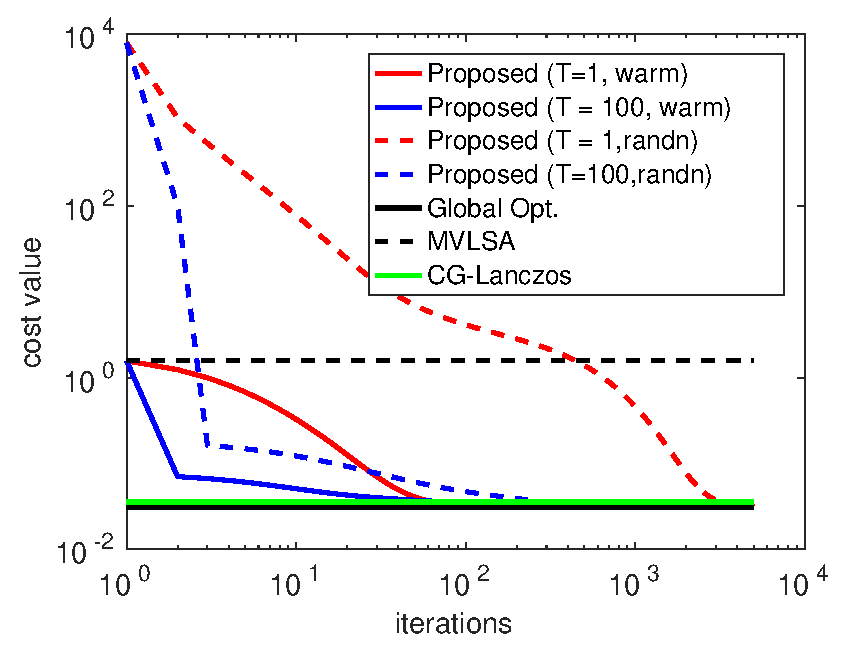
\includegraphics[width=6.15cm]{lambda_1.eps}
\label{fig:subfigure1}}
\subfigure[Cost v.s. iter. $(r)$; large case.]{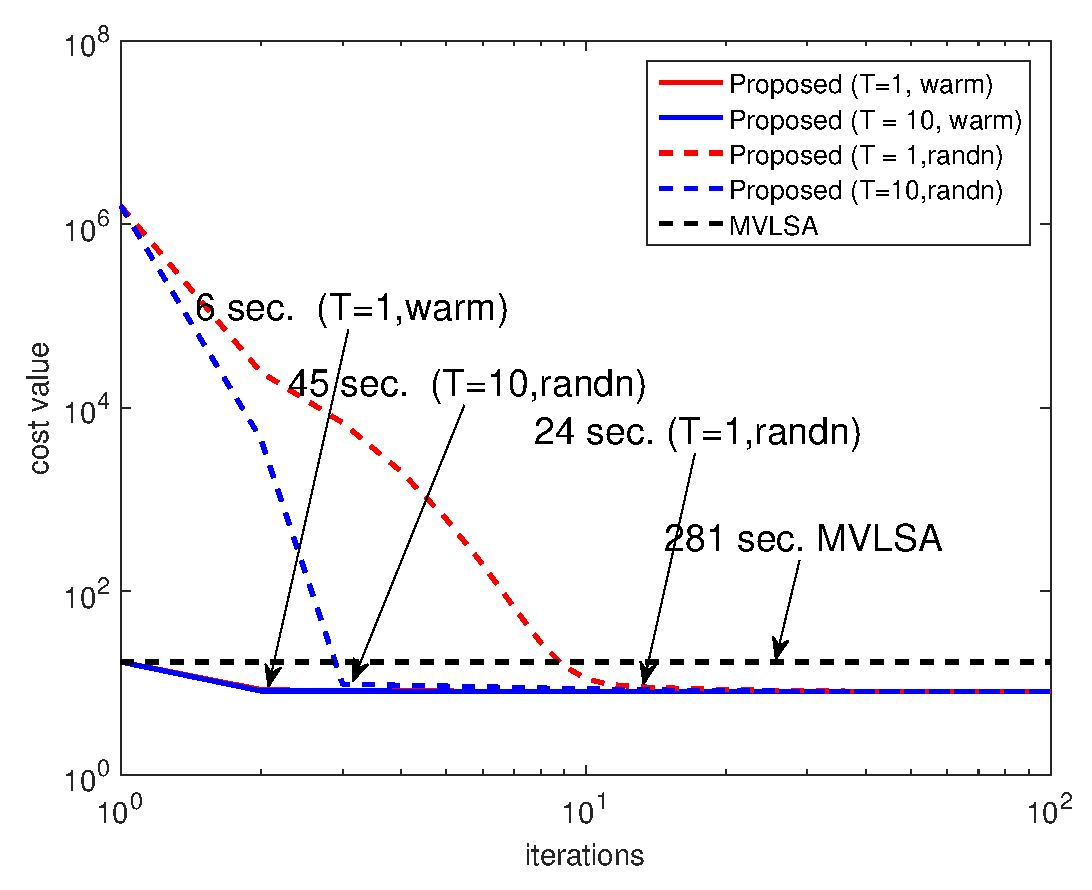
\includegraphics[width=6.15cm]{cost_large.eps}
\label{fig:subfigure3}}
\caption{Performance of the algorithms under various settings.}
\end{figure}

\begin{figure}[ht]
\centering

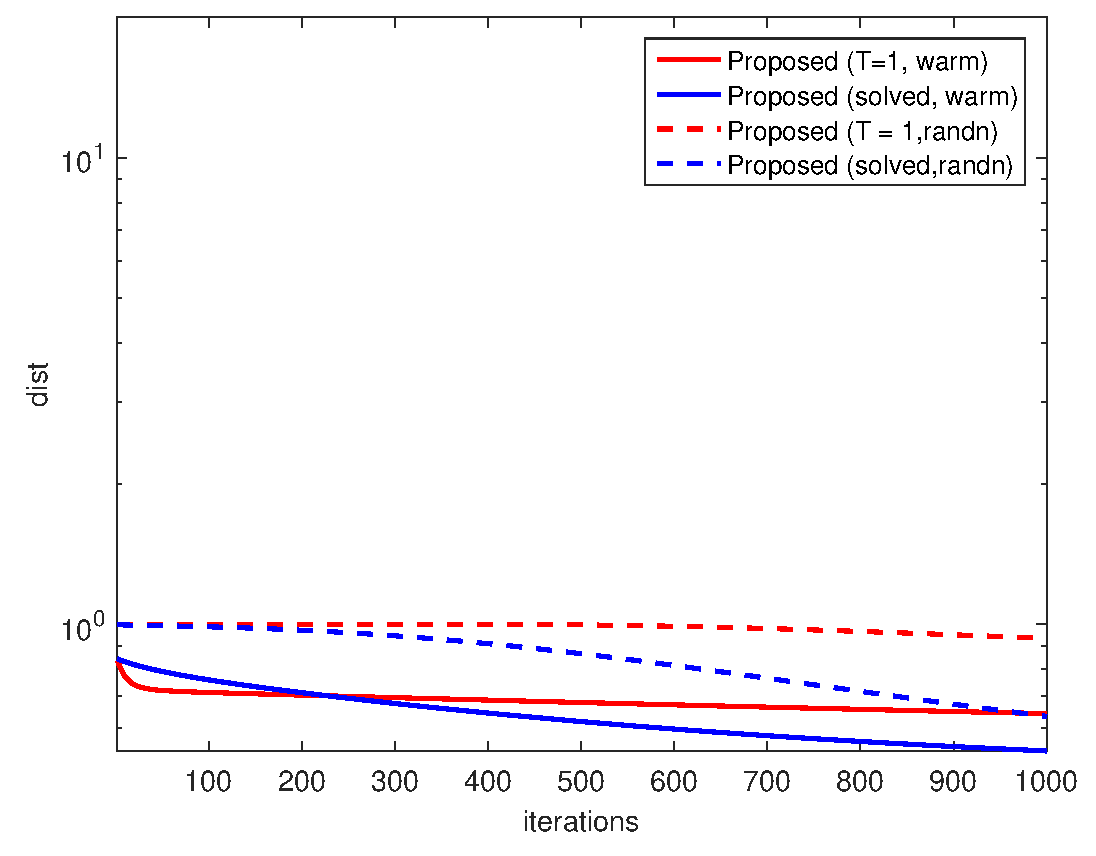
\includegraphics[width=6cm]{dist_lambda_1.eps}

\caption{Linear rate of subspace dist. v.s. iter. $(r)$}\label{fig:subfigure2}
\end{figure}

Fig.~\ref{fig:subfigure2} shows the ${\rm dist}\left({\cal R}({\bm G}^{(r)}),{\cal R}_K({\bm M})\right)$'s obtained by the proposed algorithm under various settings against $r$.
The settings are the same as those in Fig. 1(a) in the manuscript.
We see that if the subproblem w.r.t. ${\bm Q}_i$ is solved, the algorithm does give a linear convergence rate, as we stated in Theorem~\ref{thm:main}. Even we restrict the inner loop to $T=10$ iterations, the rate is still empirically linear, but with a slightly worse slope.


{\blue The simulations with outliers go from here}


\subsection{Real-Data Validation}
We test the algorithms on a large-scale multilingual dataset.
The views are extracted from a large word co-occurrence matrix, which is available at \url{https://sites.google.com/a/umn.edu/huang663/research}.
The original data contains words of three languages, namely, English, Spanish, and French,
and all the words are defined by co-occurences with other words.
We use the English words to form our first view, ${\bm X}_1$, which contains $L=183,034$ words and each word is defined by $M_i=100,000$ features (co-occurrences). Note that ${\bm X}_1$ is sparse -- only $1.21\%$ of its entries are non-zeros.
Using a dictionary, we pick out the translations of the English words contained in ${\bm X}_1$ in Spanish and French to form ${\bm X}_2$ and ${\bm X}_3$, respectively.
Note that many English words do not have a corresponding word in Spanish (or French).
In such cases, we simply let ${\bm X}_i(\ell,:)={\bm 0}$ for $i=2$ (or $i=3$),
resulting in sparser ${\bm X}_2$ and ${\bm X}_3$.


Our objective is to find ${\bm G}$ whose rows are the low-dimensional embeddings of the English words.
To evaluate the output, we use the evaluation tool provided at {wordvectors.org} \cite{faruqui-2014:SystemDemo}, which runs several word embedding tasks to evaluate a set of given embeddings. Simply speaking, the tasks compare the algorithm-learned
embeddings with the judgment of humans and yield high scores if the embeddings are consistent with the humans. The scores are between zero and one,
and a score equal to one means a perfect alignment between the learned result and human judgment.
We use the result of MVLSA with $P=640$ as benchmark. 
The result of applying SVD to ${\bm X}_1$ without considering different languages is also presented.
We apply the proposed algorithm warm started by MVLSA and set $T=1$.
We run two versions of our algorithm. The first one uses $g_i(\cdot)=\|\cdot\|_F^2$
for $i=1,2,3$.
The second one uses $g_i(\cdot)=0.05\|\cdot\|_{2,1}$ for $i=2,3$.
The reason for adding $\ell_2/\ell_1$ mixed norm regularization to the French and Spanish views
is towfold:
First, the languages are effectively `fat matrices' and thus need to use a column-selective regularizer.
Second, the $\ell_2/\ell_1$ norm promotes row sparsity of $\Q_i$ and thus performs feature selection on $\X_2$ and $\X_3$ -- this physically means that we aim at selecting the most useful features from the other languages to help enhance English word embeddings.


Tables~\ref{tab:K50} and \ref{tab:K100} show the word embedding results using $K=50$ and $K=100$, respectively.
We see that using the information from multiviews does help in improving the word embeddings:
For $K=50$ and $K=100$, the multiview approaches perform better relative to SVD in 11 and 8 tasks out of 12 tasks. 
In addition, the proposed algorithm with the regularizer $g_i(\cdot)=\|\cdot\|_F^2$ gives similar or slightly better in average on both experiments compared to MVLSA.
The proposed algorithm with the feature-selective regularizer ($g_i(\cdot)=\lambda_i\|\cdot\|_{2,1}$) gives the best evaluation results on both experiments -- this suggests that for large-scale multiview analysis, feature selection is much meaningful.


% Table generated by Excel2LaTeX from sheet 'Sheet1'
% Table generated by Excel2LaTeX from sheet 'Sheet1'
\begin{table}[htbp]
  \centering
  \caption{Evaluation on 12 word embedding tasks; $K=50$.}
  	\resizebox{\linewidth}{!}{\footnotesize
        \begin{tabular}{c|c|c|c|c}
        \hline
        \hline
        \multirow{2}[4]{*}{Task} & \multicolumn{4}{c}{Algorithm ($K=50$)}\\
    \cline{2-5}          & svd   & MVLSA & Proposed ($\|\cdot\|_F^2$) & Proposed  ($\|\cdot\|_{2,1}$)\\
        \hline
        \hline
        EN-WS-353-SIM & 0.63  & \textbf{0.69} & 0.67  & 0.68\\
        \hline
        EN-MC-30 & 0.56  & 0.63  & 0.63  & \textbf{0.64}\\
        \hline
        EN-MTurk-771 & 0.54  & 0.58  & 0.59  & \textbf{0.60}\\
        \hline
        EN-MEN-TR-3k & 0.67  & 0.66  & 0.67  & \textbf{0.68}\\
        \hline
        EN-RG-65 & 0.51  & 0.53  & 0.55  & \textbf{0.58}\\
        \hline
        EN-MTurk-287 & \textbf{0.65} & 0.64  & \textbf{0.65} & 0.64\\
        \hline
        EN-WS-353-REL & 0.50  & 0.51  & 0.53  & \textbf{0.55}\\
        \hline
        EN-VERB-143 & 0.21  & \textbf{0.22} & 0.21  & 0.21\\
        \hline
        EN-YP-130 & 0.36  & 0.39  & 0.38  & \textbf{0.41}\\
        \hline
        EN-SIMLEX-999 & 0.31  & \textbf{0.42} & 0.41  & 0.39\\
        \hline
        EN-RW-STANFORD & 0.39  & \textbf{0.43} & \textbf{0.43} & \textbf{0.43}\\
        \hline
        EN-WS-353-ALL & 0.56  & 0.59  & 0.59  & \textbf{0.60}\\
        \hline
        \hline
        average & 0.49  & 0.52  & 0.53  & \textbf{0.54}\\
        \hline
        median & 0.53  & 0.56  & 0.57  & \textbf{0.59}\\
        \hline
        \hline
        \end{tabular}%
    
    }%
  \label{tab:K50}%
\end{table}%

% Table generated by Excel2LaTeX from sheet 'July31'
\begin{table}[htbp]
  \centering
  \caption{Evaluation on 12 word embedding tasks; $K=100$.}  
  	\resizebox{\linewidth}{!}{\footnotesize
    \begin{tabular}{c|c|c|c|c}
    \hline
    \hline
    \multirow{2}[4]{*}{Task} & \multicolumn{4}{c}{Algorithm ($K=100$)}\\
\cline{2-5}          & svd   & MVLSA & Proposed ($\|\cdot\|_F^2$) & Proposed  ($\|\cdot\|_{2,1}$)\\
    \hline
    \hline
    EN-WS-353-SIM & 0.68  & \textbf{0.72} & 0.71  & \textbf{0.72}\\
    \hline
    EN-MC-30 & 0.73  & 0.68  & 0.72  & \textbf{0.74}\\
    \hline
    EN-MTurk-771 & 0.59  & 0.60  & 0.60  & \textbf{0.61}\\
    \hline
    EN-MEN-TR-3k & \textbf{0.72} & 0.70  & 0.70  & 0.71\\
    \hline
    EN-RG-65 & \textbf{0.68} & 0.63  & 0.64  & \textbf{0.68}\\
    \hline
    EN-MTurk-287 & 0.61  & \textbf{0.66} & 0.65  & 0.64\\
    \hline
    EN-WS-353-REL & \textbf{0.57} & 0.54  & 0.55  & 0.56\\
    \hline
    EN-VERB-143 & 0.19  & 0.28  & 0.27  & \textbf{0.29}\\
    \hline
    EN-YP-130 & 0.42  & 0.41  & 0.41  & \textbf{0.45}\\
    \hline
    EN-SIMLEX-999 & 0.34  & \textbf{0.42} & 0.41  & 0.41\\
    \hline
    EN-RW-STANFORD & 0.44  & \textbf{0.46} & 0.45  & \textbf{0.46}\\
    \hline
    EN-WS-353-ALL & \textbf{0.62} & \textbf{0.62} & \textbf{0.62} & \textbf{0.62}\\
    \hline
    \hline
    average & 0.55  & 0.56  & 0.56  & \textbf{0.58}\\
    \hline
    median & 0.60  & 0.61  & 0.61  & \textbf{0.62}\\
    \hline
    \hline
    \end{tabular}%
    }
  \label{tab:K100}%
\end{table}%


\section{Conclusion}

In this work, we revisited the MAX-VAR GCCA problem with an eye towards scenarios involving large-scale and sparse data. 
The proposed AO-based approach is memory-efficient and has light per-iteration computational complexity if the views are sparse, and is thus suitable for dealing with big data.
A thorough convergence analysis was presented, showing that the proposed algorithmic framework
guarantees global optimality for the MAX-VAR GCCA problem when the subproblems in the AO framework are exactly solved in each iteration. In addition, when one subproblem is only inexactly solved, global convergence to a KKT point
was also shown. Simulations and careful experiments with large-scale multi-lingual data showed that the performance of the proposed algorithm is promising in dealing with large and sparse multiview data.



\ifplainver
    \section*{Appendix}
    \renewcommand{\thesubsection}{\Alph{subsection}}
\else
\appendices
\fi



\section{Proof of Proposition~\ref{lem:monotonicity}}
Before proving the Proposition, let us first simplify the notation. Recall that we have defined ${\bm Q}=[{\bm Q}_1^T,\ldots,{\bm Q}_I^T]^T$ as a collection 
of $\Q_i$'s
and we define
$F({\bm G},{\bm Q}) = \sum_{i=1}^{I}\frac{1}{2}\left\|{\bm X}_i{\bm Q}_i-{\bm G}\right\|_F^2 + \sum_{i=1}^Ig_i(\Q_i),$
and the continuous differentiable part of the above as
$f({\bm G},{\bm Q}) = \sum_{i=1}^{I}\frac{1}{2}\left\|{\bm X}_i{\bm Q}_i-{\bm G}\right\|_F^2.$
Since the algorithm is essentially a two-block alternating optimization (i.e., ${\bm Q}_i$ for all $i$ are updated simultaneously), the above notation suffices to describe the updates.
We also define
\begin{align*}
u_Q\left(\Q;\hat{\bm G},\hat{\bm Q}\right) = &f(\hat{\bm G},\hat{\bm Q}) + \sum_{i=1}^I (\nabla_{{\bm Q}_i} f(\hat{\bm G},\hat{\bm Q}))^T({\bm Q}_i-\hat{\bm Q}_i)\\
&+ \sum_{i=1}^I\frac{1}{2\alpha_i}\|{\bm Q}_i-\hat{\bm Q}\|_F^2+ \sum_{i=1}^Ig_i(\Q_i);
\end{align*}
i.e., $u_Q\left({\bm Q};\hat{\bm G},\hat{\bm Q}\right)$ is an approximation of $F({\bm G},{\bm Q})$
locally at the point $(\hat{\bm G},\hat{\bm Q}_i)$, and
we also define
\begin{equation*}
\begin{aligned}
\tilde{u}_Q\left(\Q;\hat{\bm G},\hat{\bm Q}\right) = &f(\hat{\bm G},\hat{\bm Q})
+ \sum_{i=1}^I (\nabla_{{\bm Q}_i} f(\hat{\bm G},\hat{\bm Q}))^T({\bm Q}_i-\hat{\bm Q}_i)\\& + \sum_{i=1}^I\frac{1}{2\alpha_i}\|{\bm Q}_i-\hat{\bm Q}\|_F^2;
\end{aligned}
\end{equation*}
i.e., $\tilde{u}_Q\left(\Q;\hat{\bm G},\hat{\bm Q}\right)$ is an approximation of $f({\bm G},{\bm Q})$
locally at the point $(\hat{\bm G},\hat{\bm Q}_i)$.
%By the definition o
%\begin{equation*}
%	\nabla_{{\bm Q}_i} f\left(\hat{\bm G},\hat{\bm Q}\right) = \nabla_{{\bm Q}_i} f(\hat{\bm G},{\bm Q})|_{{\bm Q}_i=\hat{\bm Q}_i}.
%\end{equation*}
We see that,
\begin{equation}\label{eq:gradequal}
\begin{aligned}
	&\nabla_{{\bm Q}_i} f\left(\hat{\bm G},\hat{\bm Q}\right)=\nabla_{{\bm Q}_i} \tilde{u}\left(\hat{\bm Q};\hat{\bm G},\hat{\bm Q}\right),\\
	& \nabla_{{\bm Q}} f\left(\hat{\bm G},\hat{\bm Q}\right) + \partial_{\Q} g(\Q) = \nabla_{{\bm Q}}\tilde{u}\left(\hat{\bm Q};\hat{\bm G},\hat{\bm Q}\right) + \partial_{\Q} g(\Q),
\end{aligned}
\end{equation}
where $\nabla_{{\bm Q}} f\left(\hat{\bm G},\hat{\bm Q}\right)$, $\partial_{\Q} g(\Q)$ and $\nabla_{{\bm Q}}\tilde{u}\left(\hat{\bm Q};\hat{\bm G},\hat{\bm Q}\right)$ follow the definitions in \eqref{eq:definie_diff}.
Since $\nabla_{{\bm Q}_i} f({\bm G},{\bm Q})$ is $L_i$-Lipschitz continuous w.r.t. ${\bm Q}_i$ and $\alpha_i\leq 1/L_i$ for all $i$, we see that
\begin{equation}\label{eq:gleqf}
	u_Q\left({\bm Q};\hat{\bm G},\hat{\bm Q}\right)\geq F\left(\hat{\bm G},{\bm Q}\right),~\forall~{\bm Q},
\end{equation}
where the equality holds if and only if ${\bm Q}_i = \hat{\bm Q}_i$ for all $i$, i.e.,
\begin{equation}\label{eq:geqf}
u_Q\left(\hat{\bm Q};\hat{\bm G},\hat{\bm Q}\right) = F\left(\hat{\bm G},\hat{\bm Q}\right).
\end{equation}
Now, let us denote by ${\bm Q}^{(r,t)}$ (where $0\leq t\leq T$) the solution of ${\bm Q}$
after $t$ gradient updates when ${\bm G}^{(r)}$ is fixed, where $r$ is the iteration index of the outer loop.
With the above notation, we have ${\bm Q}^{(r,0)}={\bm Q}^{(r)}$ and ${\bm Q}^{(r,T)}={\bm Q}^{(r+1)}$.
Also, it can be seen that the update of $\{{\bm Q}_i\}$ can be written as
\begin{equation}\label{eq:updateQ}
\begin{aligned}
	{\bm Q}_i^{(r,t+1)}&= \texttt{prox}_{g}\left({\bm Q}_i^{(r,t)} - \alpha_i \nabla_{{\bm Q}_i} f\left({\bm G}^{(r)},{\bm Q}^{(r,t)}\right)\right)\\
	                 &= \arg\min_{{\bm Q}_i}~u_{Q}\left( {\bm Q};{\bm G}^{(r)},{\bm Q}^{(r,t)} \right).
\end{aligned}
\end{equation}


Similarly, we define
\begin{align*}
u_G\left(\G;\hat{\bm G},\hat{\bm Q}\right) = &f(\hat{\bm G},\hat{\bm Q}) +  (\nabla_{\G} f(\hat{\bm G},\hat{\bm Q}))^T(\G-\hat{\bm G})\\
& + \frac{1}{2\gamma}\left\|\G-\hat{\G}\right\|_F^2+ \sum_{i=1}^Ig_i(\hat{\Q_i}),
\end{align*}
where the last term is constant if $\Q$ is fixed.
We also have the following hold:
\begin{equation}\label{eq:Ggradequal}
\begin{aligned}
	&\nabla_{\G} f\left(\hat{\bm G},\hat{\bm Q}\right)=\nabla_{\G} {u}\left(\hat{\bm G};\hat{\bm G},\hat{\bm Q}\right).
\end{aligned}
\end{equation}

The update rule of $\G$ in Algorithm~\ref{algo:AltCCA} can be re-expressed as follows:
\begin{align*}
 \G \in & \arg\min_{\G^T\G={\bm I}}~\left\|\G - \left((1-\gamma)\hat{\G}+\gamma \sum_{i=1}^I\nicefrac{\X_i\Q_i}{I}\right)\right\|_F^2 \\
\Leftrightarrow  \G  \in & \arg\min_{\G^T\G={\bm I}}~\left\|\G - \left(\hat{\G}-\gamma \nabla_{\G} f\left(\hat{\bm G},\hat{\bm Q}\right)\right)\right\|_F^2\\
\Leftrightarrow   \G  \in & \arg\min_{\G^T\G={\bm I}}~u_G\left(\G;\hat{\bm G},\hat{\bm Q}\right)
\end{align*}
Since $\nabla_{\G} f({\bm G},{\bm Q})$ is $1$-Lipschitz continuous w.r.t. $\G$ and $\gamma\leq 1$, we see that
\begin{equation}\label{eq:ugleqf}
	u_G\left({\bm G};\hat{\bm G},\hat{\bm Q}\right)\geq F\left({\bm G},\hat{\bm Q}\right),~\forall~{\bm G},
\end{equation}
and
\begin{equation}\label{eq:ugeqf}
	u_G\left(\hat{\bm G};\hat{\bm G},\hat{\bm Q}\right)= F\left(\hat{\bm G},\hat{\bm Q}\right).
\end{equation}
Using the above notations, Algorithm~\ref{algo:AltCCA} boils down to
\begin{subequations}
\begin{align}
{\bm Q}_i^{(r,t+1)}&= \arg\min_{{\bm Q}_i}~u_{Q}\left( {\bm Q};{\bm G}^{(r)},{\bm Q}^{(r,t)} \right),\quad t=0,\ldots, T-1 \label{eq:q_update_u}\\
\G^{(r+1)} &\in \arg\min_{\G^T\G={\bm I}}~u_G\left(\G;{\bm G}^{(r)},{\bm Q}^{(r,T)}\right). \label{eq:g_update_u}
\end{align}
\end{subequations}

\bigskip

Note that the following holds:
\begin{subequations}\label{eq:mono}
\begin{align}
         F\left({\bm G}^{(r)},{\bm Q}^{(r)}\right) & = u_Q(\Q^{(r)};{\bm G}^{(r)},{\bm Q}^{(r)}) \label{eq:mono1}\\
                                                   & \geq u_Q(\Q^{(r,1)};{\bm G}^{(r)},{\bm Q}^{(r,0)}) \label{eq:mono11}\\
                                                   & \geq F\left({\bm G}^{(r)},{\bm Q}^{(r,1)}\right) \label{eq:mono12}\\
                                                   & = u_Q(\Q^{(r,1)};{\bm G}^{(r)},{\bm Q}^{(r,1)}) \label{eq:mono13}\\
                                                   & \geq u_Q(\Q^{(r,2)};{\bm G}^{(r)},{\bm Q}^{(r,1)}) \label{eq:mono14}\\
                                                   &\vdots\\
%                                                   & \geq u_Q(\Q^{(r,t)};{\bm G}^{(r)},{\bm Q}^{(r,t-1)}) \label{eq:mono2}\\
                                                   & \geq u_Q(\Q^{(r+1)};{\bm G}^{(r)},{\bm Q}^{(r,T-1)}) \label{eq:mono3}\\
                                                   &\geq F\left({\bm G}^{(r)},{\bm Q}^{(r+1)}\right) \label{eq:mono4}\\
                                                   &= u_G\left({\bm G}^{(r)};{\bm G}^{(r)},{\bm Q}^{(r+1)}\right) \label{eq:mono5}\\
												   &\geq u_G\left({\bm G}^{(r+1)};{\bm G}^{(r)},{\bm Q}^{(r+1)}\right) \label{eq:mono6}\\
												   &\geq F\left({\bm G}^{(r+1)},{\bm Q}^{(r+1)}\right), \label{eq:mono7}
\end{align}
\end{subequations}
where \eqref{eq:mono1} holds because of \eqref{eq:geqf}, \eqref{eq:mono11}-\eqref{eq:mono3} hold by invoking the update rule \eqref{eq:q_update_u} and the properties in \eqref{eq:gleqf} and \eqref{eq:geqf},
\eqref{eq:mono4} holds because of \eqref{eq:gleqf},
\eqref{eq:mono5} holds due to \eqref{eq:ugeqf},
\eqref{eq:mono6} is due to the fact that \eqref{eq:g_update_u} is optimally solved,
and \eqref{eq:mono7} holds because of \eqref{eq:ugleqf}.

%where \eqref{eq:mono1_1} holds because gradient descent does not increase $f\left({\bm G}^{(r)},{\bm Q}\right)$ for $t=0,1,\ldots,T$,
%\eqref{eq:mono3} holds since ${\bm Q}^{(r,T)}={\bm Q}^{(r+1)}$,
%and \eqref{eq:mono4} holds since ${\bm G}$ is updated via solving
%\begin{equation}\label{eq:Grule}
%{\bm G}^{(r+1)}=\arg\min_{{\bm G}^T{\bm G}={\bm I}}~f\left({\bm G},{\bm Q}^{(r+1)}\right).
%\end{equation}
%This completes the proof of the first part.

\bigskip

Next, we show that every limit point is a KKT point.
Assume that there exists a convergent subsequence of $\{{\bm G}^{(r)},{\bm Q}^{(r)}\}_{r=0,1,\ldots}$,
whose limit point is $({\bm G}^\ast,{\bm Q}^\ast)$ and the subsequence is indexed by $\{r_j\}_{j=1,\ldots,\infty}$.
We have the following chain of inequalities:
\begin{subequations}\label{eq:u_Q}
\begin{align}
         u_Q\left({\bm Q};{\bm G}^{(r_j)},{\bm Q}^{(r_j)}\right) &\geq u_Q\left({\bm Q}^{(r_j,1)};{\bm G}^{(r_j)},{\bm Q}^{(r_j)}\right) \label{eq:cmin1}\\
%				                               &\geq f\left({\bm G}^{(r_j)},{\bm Q}^{(r_j,1)}\right)  \label{eq:cmin2}\\
%				                               & =  g\left({\bm Q}^{(r_j,1)};{\bm G}^{(r_j)},{\bm Q}^{(r_j,1)}\right) \label{eq:cmin21}\\
%				                               &\geq g\left({\bm Q}^{(r_j,2)};{\bm G}^{(r_j)},{\bm Q}^{(r_j,1)}\right) \label{eq:cmin22}\\
%				                               &\vdots \nonumber\\
				                               &\geq u_Q\left({\bm Q}^{(r_j,T)};{\bm G}^{(r_j)},{\bm Q}^{(r_j,T-1)}\right) \label{eq:cmin23}\\
				                              &\geq F({\bm G}^{(r_j)},{\bm Q}^{(r_j+1)})\label{eq:cmin24}\\					
                                               &\geq F\left({\bm G}^{(r_j+1)},{\bm Q}^{(r_j+1)}\right)  \label{eq:cmin3}\\
											  &\geq F\left({\bm G}^{(r_{j+1})},{\bm Q}^{(r_{j+1})}\right)  \label{eq:cmin4}\\
											   & = u_Q\left({\bm Q}^{(r_{j+1})};{\bm G}^{(r_{j+1})},{\bm Q}^{(r_{j+1})}\right), \label{eq:cmin5}
\end{align}
\end{subequations}
where \eqref{eq:cmin1} holds because of the update rule in \eqref{eq:q_update_u},
\eqref{eq:cmin23} holds by repeating the arguments in \eqref{eq:mono11}-\eqref{eq:mono3},
\eqref{eq:cmin3} follows \eqref{eq:mono7},
and \eqref{eq:cmin5} is again because of the way that we construct $u_Q({\bm Q};{\bm G}^{(r_{j+1)}},{\bm Q}^{(r_{j+1})})$.

%\eqref{eq:cmin2} holds due to \eqref{eq:gleqf},
%\eqref{eq:cmin21} holds because of \eqref{eq:geqf},
%the chain of \eqref{eq:cmin22}-\eqref{eq:cmin24} follows from the same reasons as the above,
%\eqref{eq:cmin3} is by virtue of the update rule in \eqref{eq:Grule},
%and from the monotonicity that we established in \eqref{eq:mono},
%and \eqref{eq:cmin5} is again because of the way that we construct $g({\bm Q};{\bm G}^{(r_{j+1)}},{\bm Q}^{(r_{j+1})})$.



Taking $j\rightarrow \infty$, and by continuity of $u_Q(\cdot)$, we have
\begin{equation}
	    u_Q({\bm Q};{\bm G}^{\ast},{\bm Q}^\ast) \geq  u_Q({\bm Q}^\ast;{\bm G}^{\ast},{\bm Q}^\ast),
\end{equation}
i.e., ${\bm Q}^{\ast}$ is a minimum of $u_Q({\bm Q};{\bm G}^{\ast},{\bm Q}^\ast)$.
Consequently, ${\bm Q}^{\ast}$ satisfies the conditional KKT conditions, i.e.,
\begin{equation}
	 {\bm 0} \in  \nabla_{{\bm Q}} \tilde{u}_Q({\bm Q}^\ast;{\bm G}^{\ast},{\bm Q}^\ast) + \partial_{\Q}g(\Q^\ast),
\end{equation}
which also means that the following holds:
\begin{equation}\label{eq:QKKT}
	     {\bm 0} \in \nabla_{{\bm Q}_i} f({\bm G}^{\ast},{\bm Q}^\ast) + \partial_{\Q}g(\Q^\ast) ,
\end{equation}
following \eqref{eq:gradequal}.

We now show that $\Q^{(r_j,t)}$ for $t=1,\ldots,T$ also converges to $\Q^\ast$.
Indeed, we have
\begin{align*}
u_Q(\Q^{(r_{j+1})};\G^{(r_{j+1})},\Q^{(r_{j+1})})&\leq u_Q(\Q^{(r_j,1)};\G^{(r_j)},\Q^{(r_j)})\\
&\leq u_Q(\Q^{(r_j)};\G^{(r_j)},\Q^{(r_j)}) ,
\end{align*}
where the first inequality was derived from \eqref{eq:u_Q}.
Taking $j\rightarrow \infty$, we see that
$ u_Q(\Q^{\ast};\G^{\ast},\Q^{\ast})\leq u_Q(\Q^{(r_j,1)};\G^{\ast},\Q^{\ast})\leq u_Q(\Q^{\ast};\G^{\ast},\Q^{\ast}) , $
which implies that
$u_Q(\Q^{(r_j,1)};\G^{\ast},\Q^{\ast})= u_Q(\Q^{\ast};\G^{\ast},\Q^{\ast})\leq u_Q(\Q;\G^{\ast},\Q^{\ast}).$
On the other hand, the problem in \eqref{eq:q_update_u} has a unique minimizer when $g_i(\cdot)$ is convex closed function \cite{parikh2013proximal},
which means that $\Q^{(r_j,1)}\rightarrow \Q^{\ast}$. By recursion, we can show that
$\Q^{(r_j,t)}$ for $t=1,\ldots,T$ (where $T$ is finite) also converges to $\Q^\ast$ using the same argument.
Consequently, we have
\begin{equation}\label{eq:q_rj+1}
\Q^{(r_j,T)} = \Q^{(r_j+1)} \rightarrow \Q^\ast. 
\end{equation}


Now, we repeat the proof in \eqref{eq:u_Q} to ${\bm G}$:
\begin{subequations}\label{eq:u_G}
\begin{align}
         u_G\left({\bm G};{\bm G}^{(r_j)},{\bm Q}^{(r_j+1)}\right) &\geq u_G\left({\bm G}^{(r_j+1)};{\bm G}^{(r_j)},{\bm Q}^{(r_j+1)}\right) \\
				                              &\geq F({\bm G}^{(r_j+1)},{\bm Q}^{(r_j+1)})\\					
                                               &\geq F\left({\bm G}^{(r_j+1)},{\bm Q}^{(r_j+1)}\right)  \\
											  &\geq F\left({\bm G}^{(r_{j+1})},{\bm Q}^{(r_{j+1})}\right)  \\
											   & = u_G\left({\bm G}^{(r_{j+1})};{\bm G}^{(r_{j+1})},{\bm Q}^{(r_{j+1})}\right), 
\end{align}
\end{subequations}
Taking $j\rightarrow \infty$ and invoking \eqref{eq:q_rj+1}, we have
\[ u_G\left({\bm G};{\bm G}^{\ast},{\bm Q}^{\ast}\right) \geq u_G\left({\bm G}^{\ast};{\bm G}^{\ast},{\bm Q}^{\ast}\right),\quad \forall \G^T\G={\bm I}. \]
The above means that $\G^\ast$ satisfies the partial conditional KKT conditions w.r.t. $\G$.
%\begin{equation}\label{eq:GKKT}
%	   \begin{cases}
%	  \nabla_{{\bm G}} f({\bm G}^{\ast},{\bm Q}^\ast) - {\bm G}^\ast{\bm \Lambda}^\ast = {\bm 0},\\
%	  (\G^\ast)^T\G^\ast = {\bm I},
%	   \end{cases}
%\end{equation}
%where ${\bm \Lambda}$ is a dual variable associated with the constraint ${\bm G}^T{\bm G}={\bm I}$, and is symmetric \cite{wen2013feasible}.
Combining with \eqref{eq:QKKT}, we see that $({\bm G}^\ast,{\bm Q}^\ast)$ is a KKT point of the original problem. 

\bigskip

Now, we show the b) part.
First, we show that ${\bm Q}_i$ remains in a bounded set (the variable ${\bm G}$ is always bounded since we keep it feasible in each iteration). 
Since the objective value is non-increasing (cf. Theorem~\ref{lem:monotonicity}), if we denote the initial objective value as $V$, then $F({\bm G},{\bm Q}) \leq V$ holds in all subsequent iterations.  
Note that when ${\bm X}_i^{(0)}$ and ${\bm Q}_i^{(0)}$ are bounded, $V$ is also finite. 
In particular, we have $\left\| {\bm X}_i {\bm Q}_i - {\bm G} \right\|_F^2 + 2\sum_{i=1}^Ig_i(\Q_i) \leq 2V$
holds, which implies
\begin{equation}\label{eq:star}
  \| {\bm X}_i {\bm Q}_i \|_F \leq ( \| {\bm G} \|_F + \sqrt{2V} )
\end{equation}
by the triangle inequality.
The right-hand side of \eqref{eq:star} is finite since both terms are bounded. Denote $ ( \| {\bm G} \|_F + \sqrt{2V} )$ by $V'$. Then, we have
\begin{align*}
\| {\bm Q}_i \|_F &= \| ({\bm X}_i^T{\bm X}_i)^{-1} {\bm X}_i^T{\bm X}_i {\bm Q}_i \|_F\\
&\leq \| ({\bm X}_i^T{\bm X}_i)^{-1} {\bm X}_i^T \|_F \cdot \|{\bm X}_i {\bm Q}_i \|_F\\
&\leq V' \cdot \| ({\bm X}_i^T{\bm X}_i)^{-1} {\bm X}_i^T \|_F.
\end{align*} 
Now, by the assumption that ${\rm rank}({\bm X}_i)=M_i$, the term $\| ({\bm X}_i^T{\bm X}_i)^{-1} {\bm X}_i^T \|_F$ is bounded.  This shows that $\| {\bm Q}_i \|_F$ is bounded.
%For notational simplicity, we only show the $T=1$ case.
%The generalization to the $T\geq 1$ is straightforward.
%To show that ${\bm Q}_i$ is bounded all along the iterations, we first explicitly write out the updates:
%\begin{subequations}\label{eq:recurse}
%	\begin{align}
%	{\bm Q}_i^{(1)} &= {\bm Q}_i^{(0)} - \alpha_i\left(\frac{1}{L}{\bm X}_i^T{\bm X}_i{\bm Q}_i^{(0)} - \frac{1}{\sqrt{L}}{\bm X}_i^T{\bm G}^{(0)} \right) \\
%	{\bm Q}_i^{(2)} &= {\bm Q}_i^{(1)} - \alpha_i\left(\frac{1}{L}{\bm X}_i^T{\bm X}_i{\bm Q}_i^{(1)} - \frac{1}{\sqrt{L}}{\bm X}_i^T{\bm G}^{(1)} \right) \\
%	&\vdots \nonumber \\
%	{\bm Q}_i^{(r)} &= {\bm Q}_i^{(r-1)} - \alpha_i\left(\frac{1}{L}{\bm X}_i^T{\bm X}_i{\bm Q}_i^{(r-1)} - \frac{1}{\sqrt{L}}{\bm X}_i^T{\bm G}^{(r-1)} \right).
%	\end{align}
%\end{subequations}
%By sequentially plugging ${\bm Q}_i^{(t-1)}$ into ${\bm Q}_i^{(t)}$ from $t=1$ to $t=r$,
%we can write ${\bm Q}_i^{(r)}$ in the following recursion form:
%\begin{equation}
%\begin{aligned}
%{\bm Q}_i^{(r)} &= ({\bm I}-\frac{\alpha_i}{L}{\bm X}_i^T{\bm X}_i)^r{\bm Q}_i^{(0)} + ({\bm I}-\frac{\alpha_i}{L}{\bm X}_i^T{\bm X}_i)^{r-1}\frac{\alpha_i}{\sqrt{L}}{\bm X}_i^T{\bm G}^{(0)} \\
%&+ ({\bm I}-\frac{\alpha_i}{L}{\bm X}_i^T{\bm X}_i)^{r-2}\frac{\alpha_i}{\sqrt{L}}{\bm X}_i^T{\bm G}^{(1)} + \ldots + \frac{\alpha_i}{\sqrt{L}}{\bm X}_i^T{\bm G}^{(r)}
%\end{aligned}
%\end{equation}
%Consider the eigen-decomposition $\frac{1}{L}{\bm X}_i^T{\bm X}_i={\bm U}_{\bm X}{\bm \Lambda}_{\bm X}{\bm U}_{\bm X}^T$. Then, we have
%\[\|({\bm I}-\frac{\alpha_i}{L}{\bm X}_i^T{\bm X}_i)^r\|_F = \|{\bm U}_{\bm X}({\bm I}-{\bm \Lambda}_{\bm X})^r{\bm U}_{\bm X}^T\|_F\leq M_i\cdot (1-\alpha_i\cdot \mu_i)^r,\]
%where $\mu_i$ denotes the smallest eigenvalue of $\frac{1}{L}{\bm X}_i^T{\bm X}_i$.
%The above holds since we have $\alpha_i\leq 1/L_i \leq 1/\mu_i$.
%So, $0\leq 1-\alpha_i L_i\leq 1-\alpha_i\mu_i <1$ -- the last inequality holds since we have assumed that
%the views have full column rank and thus $\mu_i>0$.
%By the triangle inequality, we see that
%\begin{align}
%\|{\bm Q}_i^{(r)}\|_F &\leq M_i\cdot (1-\alpha_i\mu_i)^r \left\|{\bm Q}_i^{(0)}\right\|_F + M_i\cdot (1-\alpha_i\mu_i)^{r-1}\left\|\frac{\alpha_i}{\sqrt{L}}{\bm X}_i^T{\bm G}^{(0)}\right\|_F \nonumber \\
%&+ M_i\cdot (1-\alpha_i\mu_i)^{r-2}\left\|\frac{\alpha_i}{\sqrt{L}}{\bm X}_i^T{\bm G}^{(1)}\right\|_F + \ldots + \left\|\frac{\alpha_i}{\sqrt{L}}{\bm X}_i^T{\bm G}^{(r)}\right\|_F \nonumber \\
%&\leq KM_i\cdot (1-\alpha_i\mu_i)^r \left\|{\bm Q}_i^{(0)}\right\|_F + KM_i\cdot (1-\alpha_i\mu_i)^{r-1}\left\|\frac{\alpha_i}{\sqrt{L}}{\bm X}_i^T\right\|_F \nonumber \\
%&+ KM_i\cdot (1-\alpha_i\mu_i)^{r-2}\left\|\frac{\alpha_i}{\sqrt{L}}{\bm X}_i^T\right\|_F + \ldots + K\left\|\frac{\alpha_i}{\sqrt{L}}{\bm X}_i^T\right\|_F \nonumber \\
%& = KM_i (1-\alpha_i\mu_i)^r \left\|{\bm Q}_i^{(0)}\right\|_F + \sum_{t=1}^{r-1}KM_i(1-\alpha_i\mu_i)^{t}\left\|\frac{\alpha_i}{\sqrt{L}}{\bm X}_i^T\right\|_F + K\left\|\frac{\alpha_i}{\sqrt{L}}{\bm X}_i^T\right\|_F, \label{eq:bound_eq}
%\end{align}
%where the second inequality holds since \[\left\|\frac{\alpha_i}{\sqrt{L}}{\bm X}_i^T{\bm G}^{(r)}\right\|_F\leq \left\|\frac{\alpha_i}{\sqrt{L}}{\bm X}_i^T\right\|_F\left\|{\bm G}^{(r)}\right\|_F\]
%and $\left\|{\bm G}^{(r)}\right\|_F=K$.
%It is apparent that $\|{\bm Q}_i^{(r)}\|_F $ is bounded if $\alpha_i \leq 1/L_i$.
%In fact, the first and the second terms in \eqref{eq:bound_eq} is bounded since $(1-\alpha_i\mu_i)\leq 1$,
%and the third term is bounded since we assumed that ${\bm X}_i$ is bounded.
Hence, starting from a bounded ${\bm Q}_i^{(0)}$, the solution sequence $\{\{{\bm Q}_i^{(r)}\},{\bm G}^{(r)}\}$ remains in a bounded set. Since the constraints of ${\bm Q}_i$, i.e., $\mathbb{R}^{M_i\times K}$ and ${\bm G}$ are also closed sets,  $\{\{{\bm Q}_i^{(r)}\},{\bm G}^{(r)}\}$ remains in a compact set.

Now, let us denote ${\cal K}$ as the set containing all the KKT points.
Suppose the whole sequence does not converge to ${\cal K}$.
Then, there exists a convergent subsequence indexed by $\{r_j\}$ such that
$\lim_{j\rightarrow \infty} d({\cal K})\geq \gamma$
for some positive $\gamma$, where
$d({\cal K}) = \min_{{\bm Y}\in{\cal K}}~\|({\bm G},\{{\bm Q}_i\}) - {\bm Y}\|.$
Since the subsequence indexed by $\{r_j\}$ lies in a closed and bounded set as we have shown,
this subsequence has a limit point.
However, as we have shown in Theorem~\ref{lem:monotonicity}, every limit point of the solution sequence is a KKT point.
This is a contradiction.
Therefore, the whole sequence converges to a KKT point.
%\hfill $\square$

\section{Proof of Lemma~\ref{lem:z} and Theorem~\ref{thm:complexity}}\label{app:complexity}

To keep the notations simple, we prove the theorem using the $T=1$ case.
The proof of the $T\geq 2$ can be obtained in a straightforward manner. 
We first show that $Z^{(r,r+1)}\rightarrow 0$ implies that a KKT point is reached.
First, by the updating rule, we have

\begin{align}
\Q^{(r,t)} = &\arg\min_{\Q}~ \left<\nabla_{\Q}f(\Q^{(r,t-1)},\G^{(r)}),\Q -\Q^{(r,t-1)}\right> \nonumber\\
     & + \sum_{i=1}^Ig_i(\Q_i)+\sum_{i=1}^I\frac{1}{2\alpha_i}\|\Q_i-\Q_i^{(r,t-1)}\|_F^2.  \label{eq:q_arg}
\end{align}

Therefore, $\Q^{(r,t)}$ satisfies the optimality condition of the RHS, i.e.,
\begin{align*}
&{\bm 0}\in \nabla_{\Q}f(\Q^{(r,t-1)},\G^{(r)}) + \partial_{\Q}g(\Q^{(r,t)})+{\bm D}(\Q^{(r,t)}-\Q^{(r,t-1)}),
%\Rightarrow & \|\nabla_{\Q}f(\Q^{(r)},\G^{(r)}) + \partial_{\Q}r(\Q^{(r+1)}) \|_F^2 = \sum_{i=1}^I\frac{1}{\alpha_i^2}\left\|\Q_i^{(r+1)}-\Q_i^{(r)}\right\|_F^2, \label{eq:q_norm}
\end{align*}
where
${\bm D}={\rm Diag}\left(\frac{1}{\alpha_1}{\bm 1}^T_{M_1},\ldots,\frac{1}{\alpha_I}{\bm 1}^T_{M_I}\right).$
Therefore, there exists a $\partial_{\Q} g\left(\Q^{(r,t+1)}\right)$ such that
\begin{equation} \label{eq:q_norm}
\begin{aligned}
&\sum_{t=0}^{T-1}\left(\nabla_{\Q}~f\left(\Q^{(r,t)},\G^{(r)}\right) + \partial_{\Q} g\left(\Q^{(r,t+1)}\right)\right) \\
&= -\left({\bm D}(\Q^{(r)}-\Q^{(r+1)})\right).
\end{aligned}
\end{equation}
Consequently, we have
\begin{align*}
&\sum_{t=0}^{T-1}\left\|\left(\nabla_{\Q}~f\left(\Q^{(r,t)},\G^{(r)}\right) + \partial_{\Q} g\left(\Q^{(r,t+1)}\right)\right) \right\|_F^2 \rightarrow 0 \nonumber\\
&~~\Rightarrow \Q_i^{(r,t)}-\Q_i^{(r,t+1)} \rightarrow {\bm 0},~\forall~t=0,\ldots,T-1\\
&~~\Rightarrow \Q_i^{(r)}-\Q_i^{(r+1)} \rightarrow 0,
\end{align*}
which holds since $T$ is finite.
The above means that 
${\bm 0}\in \nabla_{\Q}f(\Q^{(r)},\G^{(r)}) + \partial_{\Q}g(\Q^{(r)})$
is satisfied when $Z^{r,r+1}\rightarrow 0$.


%To keep the notations simple, we prove the theorem using the $T=1$ case.
%The proof of the $T\geq 2$ can be obtained in a straightforward manner. 
%We first show that $Z^{(r,r+1)}\rightarrow 0$ implies that a KKT point is reached.
%First, by the updating rule, we have
%\begin{equation}\label{eq:q_arg}
%\Q^{(r+1)} = \arg\min_{\Q}~ \left<\nabla_{\Q}f(\Q^{(r)},\G^{(r)}),\Q -\Q^{(r)}\right> + r(\Q)+\sum_{i=1}^I\frac{1}{2\alpha_i}\|\Q_i-\Q_i^{(r)}\|_F^2. 
%\end{equation}
%Therefore, $\Q^{(r+1)}$ satisfies the optimality condition of the RHS, i.e.,
%\begin{align}
%&{\bm 0}\in \nabla_{\Q}f(\Q^{(r)},\G^{(r)}) + \partial_{\Q}r(\Q^{(r+1)})+{\bm D}(\Q^{(r+1)}-\Q^{(r)}) \nonumber \\
%\Rightarrow & \|\nabla_{\Q}f(\Q^{(r)},\G^{(r)}) + \partial_{\Q}r(\Q^{(r+1)}) \|_F^2 = \sum_{i=1}^I\frac{1}{\alpha_i^2}\left\|\Q_i^{(r+1)}-\Q_i^{(r)}\right\|_F^2, \label{eq:q_norm}
%\end{align}
%where
%\[{\bm D}={\rm Diag}\left(\frac{1}{\alpha_1}{\bm 1}^T_{M_1},\ldots,\frac{1}{\alpha_I}{\bm 1}^T_{M_I}\right).\]
%The above implies that
%\begin{align}
%\|\nabla_{\Q}f(\Q^{(r)},\G^{(r)}) + \partial_{\Q}r(\Q^{(r+1)}) \|_F^2 \rightarrow 0 \nonumber\\
%\Rightarrow \left\|\Q_i^{(r+1)}-\Q_i^{(r)}\right\|_F^2 \rightarrow 0.
%\end{align}

Now we observe the update rule of $\G$, which is equivalent to solving
\begin{equation}\label{eq:G_projgrad}
\begin{aligned}
\min_{\G^T\G=\bm I}\quad \left\|\G - \left(\G^{(r)} -\gamma \left(\nabla_{\G}~f(\G^{(r)},\Q^{(r+1)}\right)\right)\right\|_F^2.
\end{aligned}
\end{equation}
Indeed, we have
\begin{equation}\label{eq:G_grad}
\nabla_{\G}~f(\G^{(r)},\Q^{(r+1)} )= {\bm I} -\sum_{i=1}^I\nicefrac{ \X_i\Q_i^{(r+1)}}{I}.
\end{equation}
Substituting \eqref{eq:G_grad} into \eqref{eq:G_projgrad} we have
\begin{equation}\label{eq:G_P}
\begin{aligned}
\min_{\G^T\G=\bm I}\quad \left\|\G - \left((1-\gamma)\G^{(r)}+ \gamma\sum_{i=1}^I \frac{ \X_i\Q_i^{(r+1)}}{I}\right)\right\|_F^2,
\end{aligned}
\end{equation}
and the solution to the above amounts to SVD of $\bm P$.
Therefore, following the argument in \eqref{eq:q_arg}, we have
\begin{equation}\label{eq:g_arg}
\begin{aligned}
\G^{(r+1)} \in& \arg\min_{\G^T\G={\bm I}}~ <\nabla_{\G}f(\Q^{(r+1)},\G^{(r)}),\G -\G^{(r)}>\\ &+\frac{1}{2\gamma}\|\G-\G^{(r)}\|_F^2,
\end{aligned}
\end{equation}
and
\begin{align}
&\nabla_{\G}f(\Q^{(r+1)},\G^{(r)}) +\frac{1}{\gamma}\left(\G^{(r+1)} -\G^{(r)}\right) \nonumber\\
&+ \G^{(r+1)}{\bm\Lambda}^{(r+1)}={\bm 0} \nonumber\\
\Rightarrow& \left\|\nabla_{\G}f(\Q^{(r+1)},\G^{(r)})+\G^{(r+1)}{\bm \Lambda}^{(r+1)}\right\|_F^2 \nonumber\\& = \frac{1}{\gamma^2}  \left\|\G^{(r+1)} -\G^{(r)}\right\|_F^2. \label{eq:g_norm}
\end{align}
Combining \eqref{eq:g_norm} and \eqref{eq:q_norm}, we have
\begin{equation}
Z^{(r,r+1)} = \frac{1}{\gamma^2}  \left\|\G^{(r+1)} -\G^{(r)}\right\|_F^2 + \sum_{i=1}^I\frac{1}{\alpha_i^2}\left\|\Q_i^{(r+1)}-\Q_i^{(r)}\right\|_F^2.
\end{equation}
We see that $Z^{(r,r+1)}\rightarrow 0$ implies that $(\G^{(r+1)},\Q^{(r+1)})\rightarrow (\G^{(r)},\Q^{(r)})$ and that a KKT point is reached.

\bigskip

Second, we show that every iterate of $\Q$ and $\G$ gives sufficiently large decrease of the overall objective function.
Since $\nabla_{\Q_i}f(\Q,\G)$ is $L_i$-Lipschitz continuous for all $i$, we have the following:
\begin{align}
F(\Q^{(r,t+1)},\G^{(r)})&\leq f(\Q^{(r,t)},\G^{(r)}) \label{eq:24} \\
&+  <\nabla_{\Q}f(\Q^{(r,t)},\G^{(r)}),\Q -\Q^{(r)}> \nonumber\\
&  + \sum_{i=1}^Ig_i(\Q_i) + \sum_{i=1}^I\frac{L_i}{2}\left\|\Q_i-\Q_i^{(r,t)}\right\|_F^2. \nonumber
\end{align}
Since $\Q^{(r,t)}$ is a minimizer of Problem~\eqref{eq:q_arg}, we also have
\begin{align}\label{eq:25}
 &<\nabla_{\Q}f(\Q^{(r,t)},\G^{(r)}),\Q^{(r,t+1)} -\Q^{(r,t)}>+\sum_{i=1}^Ig_i(\Q_i^{(r+1)}) \nonumber\\
  &+ \sum_{i=1}^I\frac{1}{2\alpha_i}\left\|\Q_i^{(r,t+1)}-\Q_i^{(r,t)}\right\|_F^2 \leq  \sum_{i=1}^Ig_i(\Q_i^{(r,t+1)}).
\end{align}
\
Combining \eqref{eq:24} and \eqref{eq:25}, we have
\begin{equation}\label{eq:suff_q0}
\begin{aligned}
&F(\Q^{(r,t+1)},\G^{(r)}) - F(\Q^{(r,t)},\G^{(r)}) \\
& \leq -\sum_{i=1}^I\left( \frac{1}{2\alpha_i} - \frac{L_i}{2} \right)\left\|\Q_i^{(r,t+1)}-\Q_i^{(r,t)}\right\|_F^2.
\end{aligned}
\end{equation}
Summing up the above over $t=0,\ldots,T-1$, % and applying the triangle inequality, we have
\begin{equation}\label{eq:suff_q}
\begin{aligned}
& F(\Q^{(r)},\G^{(r)}) - F(\Q^{(r+1)},\G^{(r)})\\
&\geq \sum_{t=0}^{T-1}\sum_{i=1}^I\left( \frac{1}{2\alpha_i} - \frac{L_i}{2} \right)\left\|\Q_i^{(r,t+1)}-\Q_i^{(r,t)}\right\|_F^2.
\end{aligned}
\end{equation}

By the same derivation, we have
\begin{equation}\label{eq:suff_g}
\begin{aligned}
& F(\Q^{(r+1)},\G^{(r+1)}) - F(\Q^{(r+1)},\G^{(r)}) \\
& \leq -\left( \frac{1}{2\gamma} - \frac{1}{2} \right)\left\|\G^{(r+1)}-\G^{(r)}\right\|_F^2,\quad \forall \G^T\G ={\bm I}.
\end{aligned}
\end{equation}
Combining \eqref{eq:suff_q} and \eqref{eq:suff_g}, we have
\begin{equation}\label{eq:suff}
\begin{aligned}
&F(\Q^{(r)},\G^{(r)}) - F(\Q^{(r+1)},\G^{(r+1)}) \\ &\geq \left( \frac{1}{2\gamma} - \frac{1}{2} \right)\left\|\G^{(r+1)}-\G^{(r)}\right\|_F^2\\
& +\sum_{t=0}^{T-1}\sum_{i=1}^I\left( \frac{1}{2\alpha_i} - \frac{L_i}{2} \right)\left\|\Q_i^{(r,t+1)}-\Q_i^{(r,t)}\right\|_F^2.
\end{aligned}
\end{equation}
Summing up $F(\Q^{(r)},\G^{(r)})$ over $r=0,1,\ldots,J-1$, we have
Eq.~\eqref{eq:Zr}.
\begin{figure*}
\begin{align}\label{eq:Zr}
F(\Q^{(r)},\G^{(r)}) - &F(\Q^{(r+1)},\G^{(r+1)}) \nonumber\\
&\geq \sum_{r=0}^{J-1} \left( \frac{1}{2\gamma} - \frac{1}{2} \right)\left\|\G^{(r+1)}-\G^{(r)}\right\|_F^2 + \sum_{r=0}^{J-1}\sum_{t=0}^{T-1}\sum_{i=1}^I\left( \frac{1}{2\alpha_i} - \frac{L_i}{2} \right)\left\|\Q_i^{(r,t+1)}-\Q_i^{(r,t)}\right\|_F^2.\nonumber\\
& = \sum_{r=0}^{J-1} \left( \frac{1}{2\gamma} - \frac{1}{2} \right)\gamma^2\left\|\nabla_{\G}f(\Q^{(r+1)},\G^{(r)})+\G^{(r+1)}{\bm \Lambda}^{(r+1)}\right\|_F^2 \nonumber\\
&+  \sum_{r=0}^{J-1}\sum_{i=1}^I\sum_{t=0}^{T-1}\left( \frac{1}{2\alpha_i} - \frac{L_i}{2} \right) \alpha_{i}^2\left\|\nabla_{\Q_i}f(\Q^{(r,t)},\G^{(r)}) + \partial_{\Q_i}g_i(\Q^{(r,t+1)}) \right\|_F^2\geq  \sum_{r=0}^{J-1} c Z^{(r,r+1)},
\end{align}
\hrulefill
\end{figure*}
where $\alpha_{\min}=\min\{\alpha_1,\ldots,\alpha_I\}$ and
\[c = \min\left\{ \left( \frac{1}{2\gamma} - \frac{1}{2} \right)\gamma^2, \left\{\left( \frac{1}{2\alpha_i} - \frac{L_i}{2} \right) \alpha_i^2\right\}_{i=1,\ldots,I} \right\}.\]
By the definition of $J$, we have
\begin{align*}
&\frac{F(\Q^{(0)},\G^{(0)}) - F(\Q^{(J)},\G^{(J)})}{J-1}\geq \frac{\sum_{r=0}^{J-1} c Z^{(r,r+1)}}{J-1}\geq c \cdot \epsilon\\
&\quad\Rightarrow  \epsilon \leq \frac{1}{c} \frac{F(\Q^{(0)},\G^{(0)}) - \bar{F}}{J-1}\\
&\quad\Rightarrow  \epsilon \leq \frac{v}{J-1},
\end{align*} 
where $\bar{F}$ is the lower bound of the cost function and
\[v = \frac{F(\Q^{(0)},\G^{(0)}) - \bar{F}}{c}. \]
This completes the proof. 




%Second, we show that every iterate of $\Q$ and $\G$ gives sufficiently large decrease of the overall objective function.
%Since $\nabla_{\Q_i}f(\Q,\G)$ is $L_i$-Lipschitz continuous for all $i$, we have the following:
%\begin{equation}\label{eq:24}
%F(\Q^{(r+1)},\G^{(r)})\leq f(\Q^{(r)},\G^{(r)}) +  <\nabla_{\Q}f(\Q^{(r)},\G^{(r)}),\Q -\Q^{(r)}> + r(\Q^{(r+1)}) + \sum_{i=1}^I\frac{L_i}{2}\left\|\Q^{(r+1)}-\Q^{(r)}\right\|_F^2
%\end{equation} 
%Since $\Q^{(r+1)}$ is a minimizer of Problem~\eqref{eq:q_arg}, we also have
%\begin{equation}\label{eq:25}
% <\nabla_{\Q}f(\Q^{(r)},\G^{(r)}),\Q^{(r+1)} -\Q^{(r)}>+r(\Q^{(r+1)}) + \sum_{i=1}^I\frac{1}{2\alpha_i}\left\|\Q^{(r+1)}-\Q^{(r)}\right\|_F^2 \leq  r(\Q^{(r)})
%\end{equation}
%Combining \eqref{eq:24} and \eqref{eq:25}, we have
%\begin{equation}\label{eq:suff_q}
%F(\Q^{(r+1)},\G^{(r)}) - F(\Q^{(r)},\G^{(r)}) \leq -\sum_{i=1}^I\left( \frac{1}{2\alpha_i} - \frac{L_i}{2} \right)\left\|\Q^{(r+1)}-\Q^{(r)}\right\|_F^2.
%\end{equation}
%By the same derivation, we have
%\begin{equation}\label{eq:suff_g}
%F(\Q^{(r+1)},\G^{(r+1)}) - F(\Q^{(r+1)},\G^{(r)}) \leq -\left( \frac{1}{2\gamma} - \frac{1}{2} \right)\left\|\G^{(r+1)}-\G^{(r)}\right\|_F^2,\quad \forall \G^T\G ={\bm I}.
%\end{equation}
%Combining \eqref{eq:suff_q} and \eqref{eq:suff_g}, we have
%\begin{equation}\label{eq:suff}
%F(\Q^{(r)},\G^{(r)}) - F(\Q^{(r+1)},\G^{(r+1)})\geq \left( \frac{1}{2\gamma} - \frac{1}{2} \right)\left\|\G^{(r+1)}-\G^{(r)}\right\|_F^2 + \sum_{i=1}^I\left( \frac{1}{2\alpha_i} - \frac{L_i}{2} \right)\left\|\Q^{(r+1)}-\Q^{(r)}\right\|_F^2.
%\end{equation}
%Summing up $F(\Q^{(r)},\G^{(r)})$ over $r=0,1,\ldots,J-1$, we have
%\begin{align}
%F(\Q^{(r)},\G^{(r)}) - F(\Q^{(r+1)},\G^{(r+1)})&\geq \sum_{r=0}^{J-1} \left( \frac{1}{2\gamma} - \frac{1}{2} \right)\left\|\G^{(r+1)}-\G^{(r)}\right\|_F^2 + \sum_{r=0}^{J-1}\sum_{i=1}^I\left( \frac{1}{2\alpha_i} - \frac{L_i}{2} \right)\left\|\Q^{(r+1)}-\Q^{(r)}\right\|_F^2 \nonumber\\
%& = \sum_{r=0}^{J-1} \left( \frac{1}{2\gamma} - \frac{1}{2} \right)\gamma^2\left\|\nabla_{\G}f(\Q^{(r+1)},\G^{(r)})+{\bm \Lambda}^{(r+1)}\G^{(r+1)}\right\|_F^2 \nonumber\\
%&\quad\quad+  \sum_{r=0}^{J-1}\sum_{i=1}^I\left( \frac{1}{2\alpha_i} - \frac{L_i}{2} \right) \alpha^2\|\nabla_{\Q}f(\Q^{(r)},\G^{(r)}) + \partial_{\Q}r(\Q^{(r+1)}) \|_F^2\nonumber\\
%&\geq  \sum_{r=0}^{J-1} c Z^{(r,r+1)},
%\end{align}
%where
%\[c = \min\left\{ \left( \frac{1}{2\gamma} - \frac{1}{2} \right)\gamma^2, \left( \frac{1}{2\alpha_i} - \frac{L_i}{2} \right) \alpha^2 \right\}.\]
%By the definition of $J$, we have
%\begin{align}
%\frac{F(\Q^{(0)},\G^{(0)}) - F(\Q^{(J)},\G^{(J)})}{J-1}\geq \frac{\sum_{r=0}^{J-1} c Z^{(r,r+1)}}{J-1}\geq c \cdot \epsilon.
%\end{align} 
%This completes the proof. 
\section{Proof of Theorem~\ref{thm:main}}
If the subproblem with respect to (w.r.t.) ${\bm Q}_i$ is solved at outer iteration $r$,
then, by the first-order optimality condition and the assumption that ${\bm X}_i$ has full column rank, we have
\begin{equation}\label{eq:Qr1}
{\bm Q}_i^{(r+1)}=({\bm X}_i^T{\bm X}_i)^{-1}{\bm X}_i^T{\bm G}^{(r)}.
\end{equation}
Therefore, the update w.r.t. ${\bm G}$ is simply
\begin{subequations}\label{eq:MG}
\begin{align}
{\bm U}_P^{(r)}{\bm \Sigma}_P^{(r)}({\bm V}_P^{(r)})^T&={\rm svd}\left({\bm M}{\bm G}^{(r)},'{\rm econ}'\right) \label{eq:svd}\\
{\bm G}^{(r+1)}& = {\bm U}_P^{(r)}({\bm V}_P^{(r)})^T.
\end{align}
\end{subequations}
Since ${\bm V}_P^{(r)}\in\mathbb{R}^{K\times K}$ is an orthonormal matrix,
${\bm G}^{(r+1)}$ is an orthogonal basis of ${\bm M}{\bm G}^{(r)}$. In other words, there exists an invertible ${\bm \Theta}^{(r+1)}$ such that
\begin{equation}\label{eq:orthogonal}
  {\bm G}^{(r+1)}{\bm \Theta}^{(r+1)} = {\bm M}{\bm G}^{(r)}.
\end{equation}
The update rule in \eqref{eq:orthogonal}, is essentially the orthogonal iteration algorithm in \cite{GHGolub1996}.
Invoking \cite[Theorem 8.2.2]{GHGolub1996}, the proof is complete.
%\hfill $\square$

\section{Proof of Theorem~\ref{thm:main_2}}
At the $r$th iteration, ideally, we have
${\tilde{\bm Q}_i^{(r+1)}}= ({\bm X}_i^T{\bm X}_i)^{-1}{\bm X}_i^T{\bm G}^{(r)}$
if the inner problem is solved to optimality.
In practice, what we have is an inexact solution, i.e.,
${\Q}_i^{(r+1)}= ({\bm X}_i^T{\bm X}_i)^{-1}{\bm X}_i^T{\bm G}^{(r)} + {\bm W}_i^{(r)},$
where $\left\|{\bm W}_i^{(r)}\right\|_2\leq\epsilon$ is a solution mismatch term.
Hence, we see that
$\sum_{i=1}^I{\bm X}_i^T\Q_i^{(r+1)} = \M\G^{(r)} + \sum_{i=1}^I \X_i{\bm W}_i^{(r)}.$
By the algorithm, we have
\[\G^{(r+1)} =   \left(\M\G^{(r)} + \sum_{i=1}^I \X_i{\bm W}_i^{(r)}\right) {\bm \Theta}^{(r)},\]
where ${\bm \Theta}^{(r)}\in\mathbb{R}^{K\times K}$ is a full-rank matrix since SVD is a change of  bases.
Let us denote $\bm U_1$ and $\bm U_2$ as orthogonal bases of ${\cal R}_K(\M)$ and its orthogonal complement, respectively.
Then, we have
\begin{equation}
\begin{bmatrix}
\U_1^T\G^{(r+1)}\\ \U_2^T\G^{(r+1)}
\end{bmatrix}
=
\begin{bmatrix}
\bm \Lambda_1 \U_1^T\G^{(r)} + \U_1^T  \sum_{i=1}^I \X_i{\bm W}_i^{(r)} \\ \bm \Lambda_2 \U_2^T\G^{(r)} + \U_2^T  \sum_{i=1}^I \X_i{\bm W}_i^{(r)}
\end{bmatrix}
{\bm \Theta}^{(r)}.
\end{equation}
Now, we observe the equation on the top of the next page.
\begin{figure*}[t]
\begin{align}
\left\| \U_2^T\G^{(r+1)}\left( \U_1^T\G^{(r+1)} \right)^{-1}  \right\|_2 = \left\|\left(\bm \Lambda_2 \U_2^T\G^{(r)} + \U_2^T  \sum_{i=1}^I \X_i{\bm W}_i^{(r)} \right)\left(\bm \Lambda_2 \U_2^T\G^{(r)} + \U_2^T  \sum_{i=1}^I \X_i{\bm W}_i^{(r)}  \right)^{-1}\right\|_2.
\end{align}
\hrulefill
\end{figure*}
Note that we can normalize the matrix $\U_1^T  \sum_{i=1}^I \X_i{\bm W}_i^{(r)}$ as follows
\begin{equation}
   \U_1^T\sum_{i=1}^I \X_i{\bm W}_i^{(r)} = \sigma\cdot  \frac{\U_1^T  \sum_{i=1}^I \X_i{\bm W}_i^{(r)}}{\|\U_1^T \sum_{i=1}^I \X_i{\bm W}_i^{(r)}\|_2}=\sigma\tilde{\bm W}^{(r)},    
\end{equation}
where $\sigma$ is bounded by $\sigma \leq \sum_{i=1}^I\lambda_{\max}(\X_i)\epsilon$
where $\epsilon$ denotes the $2$-$norm$ upper bound of ${\bm W}_i^{(r)}$.
Using the above notations, we come up with Eq.~\eqref{eq:taylor},
\begin{figure*}[t]
\begin{align}\label{eq:taylor}
&\left\|\left(\bm \Lambda_2 \U_2^T\G^{(r)} + \U_2^T  \sum_{i=1}^I \X_i{\bm W}_i^{(r)} \right)\left(\bm \Lambda_1 \U_1^T\G^{(r)} + \U_1^T \sum_{i=1}^I \X_i{\bm W}_i^{(r)}  \right)^{-1}\right\|_2 \nonumber\\
= &\left\|\left(\bm \Lambda_2 \U_2^T\G^{(r)} + \U_2^T  \sum_{i=1}^I \X_i{\bm W}_i^{(r)} \right)\left(  \left(\bm \Lambda_1 \U_1^T\G^{(r)}\right)^{-1} + \sigma \left(\bm \Lambda_1 \U_1^T\G^{(r)}\right)^{-1} \tilde{\bm W}^{(r)}\left(\bm \Lambda_1 \U_1^T\G^{(r)}\right)^{-1} + {\cal O}(\sigma^2) \right)\right\|_2.
\end{align}
\hrulefill
\end{figure*}
where the equality is obtained by the Taylor expansion.
%Now, let us ignore the second order terms of $\sigma$ and look at the first-order terms one by one.
%First, we have
%\begin{equation}
%\begin{aligned}
%&\left\|(\bm \Lambda_2 \U_2^T\G^{(r)} )\left(\bm \Lambda_1 \U_1^T\G^{(r)}\right)^{-1} \right\|_2\\
%&\leq \frac{\lambda_{K+1}}{\lambda_K}\left\|( \U_2^T\G^{(r)} )\left( \U_1^T\G^{(r)}\right)^{-1} \right\|_2.
%\end{aligned}
%\end{equation}
%Second, we have Eq.~\eqref{eq:second_term}.
%\begin{figure*}[t]
%\begin{equation}\label{eq:second_term}
%\left\|(\bm \Lambda_2 \U_2^T\G^{(r)} )\sigma \left(\bm \Lambda_1 \U_1^T\G^{(r)}\right)^{-1} \tilde{\bm W}^{(r)}\left(\bm \Lambda_1 \U_1^T\G^{(r)}\right)^{-1}\right\|_2
%\leq \left(\sum_{i=1}^I\lambda_{\max}(\X_i)\epsilon\right) \frac{\lambda_{K+1}}{\lambda_K^2}\left\|\left(\U_1^T\G^{(r)}\right)^{-1}\right\|_2^2.
%\end{equation}
%\hrulefill
%\end{figure*}
%Third, we have
%\begin{equation}
%\begin{aligned}
%&\left\|\U_2^T  \sum_{i=1}^I \X_i{\bm W}_i^{(r)} (\bm \Lambda_1 \U_1^T\G^{(r)})^{-1} \right\|_2\\
%\leq & \left(\sum_{i=1}^I\lambda_{\max}(\X_i)\epsilon\right)\frac{1}{\lambda_K}\left\|\left(\U_1^T\G^{(r)}\right)^{-1}\right\|_2.
%\end{aligned}
%\end{equation}
%%We also have
%%\begin{equation}
%%{\blue 
%% \left\|\U_2^T  \sum_{i=1}^I \X_i{\bm W}_i^{(r)}  \sigma \left(\bm \Lambda_1 \U_1^T\G^{(r)}\right)^{-1} \tilde{\E}_K\left(\bm \Lambda_1 \U_1^T\G^{(r)}\right)^{-1}\right\|_2\leq \frac{\left(\sum_{i=1}^I\lambda_{\max}(\X_i)\epsilon\right)^2}{\lambda_{K}^2}\left\|\left(\U_1^T\G^{(r)}\right)^{-1}\right\|_2^2.}
%%\end{equation}
%%We finally have
%%\begin{equation}
%%{\blue 
%%\left\|\left(\bm \Lambda_2 \U_2^T\G^{(r)} + \U_2^T  \sum_{i=1}^I \X_i{\bm W}_i^{(r)} \right){\cal O}(\sigma^2)\right\|_2 \leq \left(\lambda_{K+1}+\sum_{i=1}^I\lambda_{\max}(\X_i)\epsilon \right){\cal O}(\sigma^2).}
%%\end{equation}
%In the derivation, we have used $\sigma \leq \sum_{i=1}^I\lambda_{\max}(\X_i)\epsilon$.

Now, let us drop the second- and higher-oder terms of $\sigma$ which are sufficiently small and `absorb' them in ${\cal O}(\|(\U_1^T\G^{(r)})^{-1}\|_2^2)$. Consequently, we come up with Eq.~\eqref{eq:finally}.
\begin{figure*}[t]
\begin{align}\label{eq:finally}
\left\| \U_2^T\G^{(r+1)}\left( \U_1^T\G^{(r+1)} \right)^{-1}  \right\|_2 
\leq \frac{\lambda_{K+1}}{\lambda_K}\left\|( \U_2^T\G^{(r)} )\left( \U_1^T\G^{(r)}\right)^{-1} \right\|_2 +\left(\sum_{i=1}^I\lambda_{\max}(\X_i)\epsilon\right) {\cal O}\left( \left\|\left(\U_1^T\G^{(r)}\right)^{-1}\right\|_2^2\right).
\end{align}
\hrulefill
\end{figure*}
Now, we show that $\left\|\left(\U_1^T\G^{(r)}\right)^{-1}\right\|_2^2$ is bounded for all $r$.
This can be seen by induction.
For $r=1$, we see that $\left\| \U_2^T\G^{(1)}\left( \U_1^T\G^{(1)} \right)^{-1}  \right\|_2$
has to be bounded since we assumed that ${\rm rank}\left(\U_1^T\G^{(0)}\right) = K$ and since
\eqref{eq:finally} holds.
Using the same argument, we see that for all $r\geq 1$, $\left( \U_1^T\G^{(1)} \right)^{-1}$ is bounded.
Let us denote an upper bound as $\beta$, i.e.,
\[\left\|\left( \U_1^T\G^{(r)} \right)^{-1}\right\|_2\leq \beta,\quad \forall r.\]
Then, we obtain Eq.~\eqref{eq:then}.
\begin{figure*}[t!]
\begin{align}\label{eq:then}
\left\| \U_2^T\G^{(r+1)}\left( \U_1^T\G^{(r+1)} \right)^{-1}  \right\|_2
\leq \frac{\lambda_{K+1}}{\lambda_K}\left\|( \U_2^T\G^{(r)} )\left( \U_1^T\G^{(r)}\right)^{-1} \right\|_2 +\left(\sum_{i=1}^I\lambda_{\max}(\X_i)\epsilon\right) {\cal O}\left( \beta^2\right).
\end{align}
\hrulefill
\end{figure*}
Using the above, we see Eq.~\eqref{eq:conclusion}  -- which completes the proof.
\begin{figure*}[t!]
\begin{align}\label{eq:conclusion}
\left\| \U_2^T\G^{(r+1)}\left( \U_1^T\G^{(r+1)} \right)^{-1}  \right\|_2
\leq \left(\frac{\lambda_{K+1}}{\lambda_K}\right)^r \left\|( \U_2^T\G^{(0)} )\left( \U_1^T\G^{(0)}\right)^{-1} \right\|_2 +\sum_{t=0}^{r-1} \left(\frac{\lambda_{K+1}}{\lambda_K}\right)^t \left(\sum_{i=1}^I\lambda_{\max}(\X_i)\epsilon\right) {\cal O}\left( \beta^2\right).
\end{align}
\hrulefill
\end{figure*}

%\section{Supplementary Experiments}






%\input{refs_aug2015.bbl}

\bibliography{refs_aug2015}
\end{document}
